\documentclass[pdftex,12pt,xcolor=svgnames]{beamer}

\mode<presentation>
{
  \usetheme{boxes}
  \usecolortheme[named=MidnightBlue]{structure}
  %\setbeamercolor{normal text}{bg=NavajoWhite!20}
  \usefonttheme{serif}
  \setbeamertemplate{navigation symbols}{}
  % Show frame number and author name in footline
  \setbeamertemplate{footline}[frame number]
  \addtobeamertemplate{footline}{\quad\textcolor{gray}{James Robert Lloyd}}{}
  % Set frame titles in small capitals
  \setbeamerfont{frametitle}{shape=\scshape,family=\rmfamily}
  \setbeamercolor{frametitle}{bg=gray!60!white,fg=black}
  % Alerted text: blue (uncomment second line if theme sets alerted text to bold)
  \setbeamercolor{alerted text}{fg=blue}
  %\setbeamerfont*{alerted text}{}
  \setbeamertemplate{bibliography item}[text] %{\hbox{\donotcoloroutermaths$\blacktriangleright$}}
  \setbeamertemplate{bibliography entry title}{}
  \setbeamertemplate{bibliography entry author}{}
  \setbeamertemplate{bibliography entry note}{}
  \setbeamertemplate{bibliography entry location}{}

}
\usepackage[english]{babel}
\usepackage[latin1]{inputenc}
\usepackage{times}
\usepackage[T1]{fontenc}
\usepackage{hyperref}
\usepackage{multimedia}
\usepackage{eepic}
\usepackage{graphicx}
%\usepackage[nohug]{latexinclude/diagrams}
\usepackage{tikz}
\usetikzlibrary{calc}

%% \newcommand{\footlineextra}[1]{
%%     \begin{tikzpicture}[remember picture,overlay]
%%         \node[yshift=1.5ex,anchor=south east] at (current page.south east)
%% {#1};
%%     \end{tikzpicture}
%% }

\newcommand{\footlineextra}[1]{
    \begin{tikzpicture}[remember picture,overlay]
        \node[xshift=-5ex,yshift=-0.5ex,anchor=south east] at (current page.south east)
             {\mbox{\tiny \textcolor{MidnightBlue}{#1}}};
    \end{tikzpicture}
}

\def\sectionframe#1{
  {
    \setbeamertemplate{footline}{\empty}
    \begin{frame}{}
      \begin{center}
        \huge\sc #1
      \end{center}
    \end{frame}
  }
}


\usepackage{etex}
%% This file provides examples of some useful macros for typesetting
% dissertations.  None of the macros defined here are necessary beyond
% for the template documentation, so feel free to change, remove, and add
% your own definitions.
%
% We recommend that you define macros to separate the semantics
% of the things you write from how they are presented.  For example,
% you'll see definitions below for a macro \file{}: by using
% \file{} consistently in the text, we can change how filenames
% are typeset simply by changing the definition of \file{} in
% this file.
% 
%% The following is a directive for TeXShop to indicate the main file
%%!TEX root = diss.tex

\newcommand{\pd}{\mbox{pd}}
\newcommand{\tr}{\mbox{tr}}
\newcommand{\mbf}[1]{\mbox{\boldmath $#1$}}
\newcommand{\deriv}[2]{\frac{\partial #1}{\partial #2}}
\newcommand{\mean}{\mathop{\mbox{mean}}}
\newcommand{\median}{\mathop{\mbox{median}}}
\newcommand{\diag}{\mbox{diag}}
\newcommand{\trace}{\mbox{trace}}
\newcommand{\st}{\mbox{st}}
\newcommand{\FF}{\tilde{F}}
\newcommand{\cut}[1]{}
\newcommand{\vn}{\varnothing}
\def\argmax{\operatornamewithlimits{arg\,max}}
\def\argmin{\operatornamewithlimits{arg\,min}}
\def\theequation{\arabic{section}.\arabic{equation}}
\def\thedefinition{\arabic{section}.\arabic{definition}}
\def\thetheorem{\arabic{section}.\arabic{theorem}}
\def\theexample{\arabic{section}.\arabic{example}}

\newcommand{\NA}{\textsc{n/a}}	% for "not applicable"
\newcommand{\eg}{e.g.,\ }	% proper form of examples (\eg a, b, c)
\newcommand{\ie}{i.e.,\ }	% proper form for that is (\ie a, b, c)
\newcommand{\etal}{\emph{et al}}

\newcommand{\expect}{\mathbb{E}}
\newcommand{\variance}{\mathbb{V}}
\newcommand{\bx}{{\bf x}}
\newcommand{\by}{{\bf y}}
\newcommand{\bX}{{\bf X}}
\newcommand{\bK}{{\bf K}}
\newcommand{\bs}{{\bf s}}
\newcommand{\bu}{{\bf u}}
\newcommand{\bff}{{\bf f}}

%\documentclass[usenames,dvipsnames]{beamer}
%\usepackage{beamerthemesplit}
%\usepackage{graphics}
%\usepackage{amsmath}
%\usepackage{rotating}
%\usepackage{array}
%\usepackage{nth}
\usepackage{xcolor}
\usepackage{textcomp}
\usepackage{listings}
%\usepackage[usenames,dvipsnames]{color}
% This is the color used for MATLAB comments below
\definecolor{MatlabDarkGreen}{rgb}{0.0,0.4,0.0}
\definecolor{Blue}{rgb}{0.0,0.0,1.0}

% For faster processing, load Matlab syntax for listings
\lstloadlanguages{Matlab}%
\lstset{language=Matlab,                        % Use MATLAB
        frame=single,                           % Single frame around code
        basicstyle=\tiny\ttfamily,             % Use small true type font
        keywordstyle=[1]\color{Blue}\bf,        % MATLAB functions bold and blue
        keywordstyle=[2]\color{Purple},         % MATLAB function arguments purple
        keywordstyle=[3]\color{Blue}\underbar,  % User functions underlined and blue
        identifierstyle=,                       % Nothing special about identifiers
                                                % Comments small dark green courier
        commentstyle=\usefont{T1}{pcr}{m}{sl}\color{MatlabDarkGreen}\tiny,
        stringstyle=\color{Purple},             % Strings are purple
        showstringspaces=false,                 % Don't put marks in string spaces
        tabsize=5,                              % 5 spaces per tab
        %
        %%% Put standard MATLAB functions not included in the default
        %%% language here
        morekeywords={xlim,ylim,var,alpha,factorial,poissrnd,normpdf,normcdf},
        %
        %%% Put MATLAB function parameters here
        morekeywords=[2]{on, off, interp},
        %
        %%% Put user defined functions here
        morekeywords=[3]{FindESS, homework_example},
        %
        morecomment=[l][\color{Blue}]{...},     % Line continuation (...) like blue comment
        numbers=left,                           % Line numbers on left
        firstnumber=1,                          % Line numbers start with line 1
        numberstyle=\tiny\color{Blue},          % Line numbers are blue
        stepnumber=50                            % Line numbers go in steps of 5
        }

% Includes a MATLAB script.
% The first parameter is the label, which also is the name of the script
%   without the .m.
% The second parameter is the optional caption.
\newcommand{\matlabscript}[2]
  {\begin{itemize}\item[]\lstinputlisting[caption=#2,label=#1]{#1.m}\end{itemize}}


\usepackage{tabularx}
\usepackage{picins}
\usepackage{tikz}

\usetikzlibrary{shapes.geometric,arrows,chains,matrix,positioning,scopes,calc}
\tikzstyle{mybox} = [draw=none, rectangle]

\definecolor{camlightblue}{rgb}{0.601 , 0.8, 1}
\definecolor{camdarkblue}{rgb}{0, 0.203, 0.402}
\definecolor{camred}{rgb}{1, 0.203, 0}
\definecolor{camyellow}{rgb}{1, 0.8, 0}
\definecolor{lightblue}{rgb}{0, 0, 0.80}
\definecolor{white}{rgb}{1, 1, 1}
\definecolor{whiteblue}{rgb}{0.80, 0.80, 1}
\definecolor{darkblue}{rgb}{0,0.08,0.45}

\newcolumntype{x}[1]{>{\centering\arraybackslash\hspace{0pt}}m{#1}}
\newcommand{\tabbox}[1]{#1}
\def\CS{\acro{CS}}

%%%%%%%%%%%%%%%%%%%%%%%%%%%%%%%%%%%%%%%%%%%
%
% Some look and feel definitions
%
%%%%%%%%%%%%%%%%%%%%%%%%%%%%%%%%%%%%%%%%%%%

\setlength{\columnsep}{0.03\textwidth}
\setlength{\columnseprule}{0.0018\textwidth}
\setlength{\parindent}{0.0cm}

%% This file provides examples of some useful macros for typesetting
% dissertations.  None of the macros defined here are necessary beyond
% for the template documentation, so feel free to change, remove, and add
% your own definitions.
%
% We recommend that you define macros to separate the semantics
% of the things you write from how they are presented.  For example,
% you'll see definitions below for a macro \file{}: by using
% \file{} consistently in the text, we can change how filenames
% are typeset simply by changing the definition of \file{} in
% this file.
% 
%% The following is a directive for TeXShop to indicate the main file
%%!TEX root = diss.tex

\newcommand{\pd}{\mbox{pd}}
\newcommand{\tr}{\mbox{tr}}
\newcommand{\mbf}[1]{\mbox{\boldmath $#1$}}
\newcommand{\deriv}[2]{\frac{\partial #1}{\partial #2}}
\newcommand{\mean}{\mathop{\mbox{mean}}}
\newcommand{\median}{\mathop{\mbox{median}}}
\newcommand{\diag}{\mbox{diag}}
\newcommand{\trace}{\mbox{trace}}
\newcommand{\st}{\mbox{st}}
\newcommand{\FF}{\tilde{F}}
\newcommand{\cut}[1]{}
\newcommand{\vn}{\varnothing}
\def\argmax{\operatornamewithlimits{arg\,max}}
\def\argmin{\operatornamewithlimits{arg\,min}}
\def\theequation{\arabic{section}.\arabic{equation}}
\def\thedefinition{\arabic{section}.\arabic{definition}}
\def\thetheorem{\arabic{section}.\arabic{theorem}}
\def\theexample{\arabic{section}.\arabic{example}}

\newcommand{\NA}{\textsc{n/a}}	% for "not applicable"
\newcommand{\eg}{e.g.,\ }	% proper form of examples (\eg a, b, c)
\newcommand{\ie}{i.e.,\ }	% proper form for that is (\ie a, b, c)
\newcommand{\etal}{\emph{et al}}

\newcommand{\expect}{\mathbb{E}}
\newcommand{\variance}{\mathbb{V}}
\newcommand{\bx}{{\bf x}}
\newcommand{\by}{{\bf y}}
\newcommand{\bX}{{\bf X}}
\newcommand{\bK}{{\bf K}}
\newcommand{\bs}{{\bf s}}
\newcommand{\bu}{{\bf u}}
\newcommand{\bff}{{\bf f}}

\usepackage{preamble}
\hypersetup{colorlinks=true,citecolor=blue}
%\pdfmapfile{+sansmathaccent.map}

\title{Structure Discovery in Nonparametric Regression through Compositional Kernel Search}


\author{
%\begin{center}
%  \begin{tikzpicture}[transform canvas={scale=0.9}] 
  \begin{scope}[yshift=0.2\textwidth]
    \begin{scope}[xshift=0cm]
      \node [mybox] (all) at (0, 0) {
        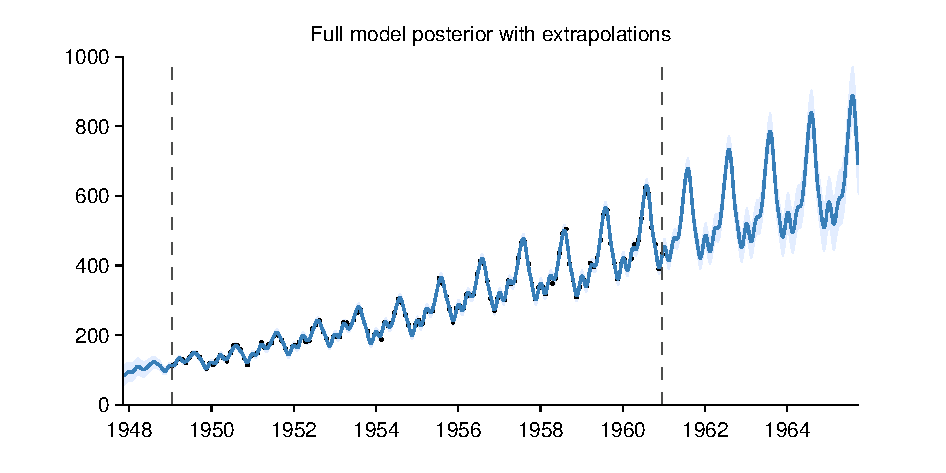
\includegraphics[width=0.8\textwidth, height=0.3\textwidth]{figures/airline/01-airline_all.pdf}
      };
    \end{scope}
  \end{scope}
  \begin{scope}[yshift=0\textwidth]
    \begin{scope}[xshift=0cm]
    \end{scope}
  \end{scope}
  \begin{scope}[yshift=0.27\textwidth]
    \begin{scope}[xshift=5cm]
        \node [mybox, below of=all] (equals) at (0, 0) {\Huge{$=$}};
    \end{scope}
  \end{scope}
  \begin{scope}[yshift=-0.1\textwidth]
    \begin{scope}[xshift=-0.3\textwidth]
      \node [mybox] (all) at (0, 0) {
        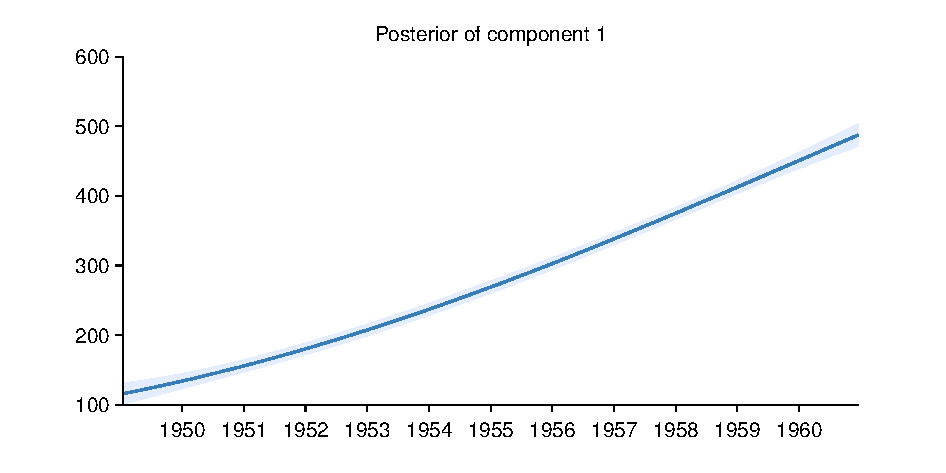
\includegraphics[width=0.5\textwidth]{figures/airline/01-airline_1.pdf}
      };
    \end{scope}
    \begin{scope}[xshift=+0.3\textwidth]
      \node [mybox] (all) at (0, 0) {
        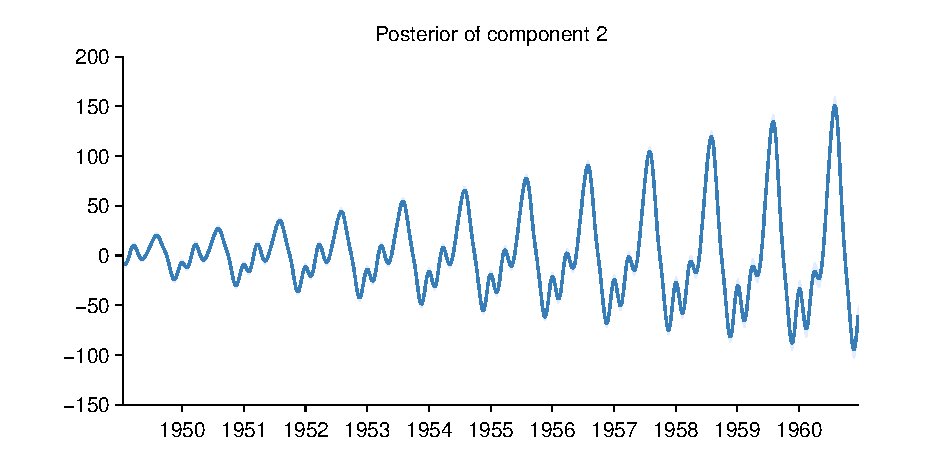
\includegraphics[width=0.5\textwidth]{figures/airline/01-airline_2.pdf}
      };
    \end{scope}
  \end{scope}
  \begin{scope}[yshift=-0.15\textwidth]
    \begin{scope}[xshift=0cm]
        \node [mybox, below of=all] (equals) at (0, 0) {\Huge{+}};
    \end{scope}
  \end{scope}
  \begin{scope}[yshift=-0.35\textwidth]
    \begin{scope}[xshift=-0.3\textwidth]
      \node [mybox] (all) at (0, 0) {
        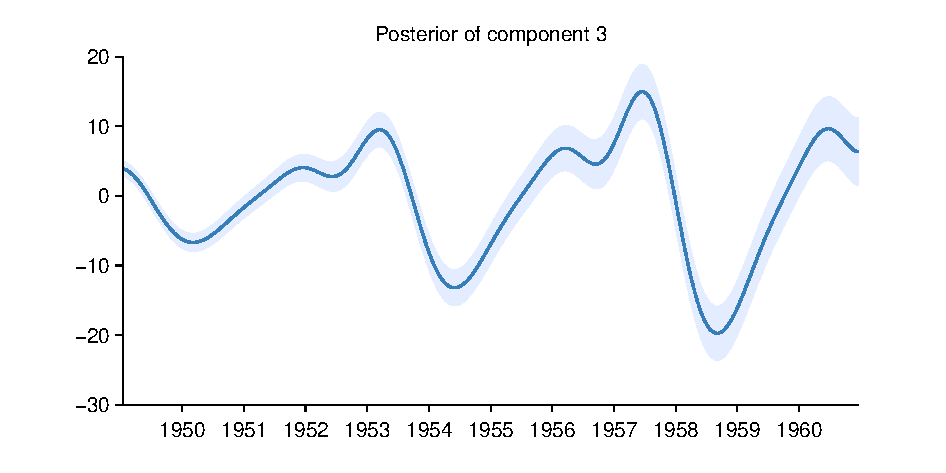
\includegraphics[width=0.5\textwidth]{figures/airline/01-airline_3.pdf}
      };
    \end{scope}
    \begin{scope}[xshift=+0.3\textwidth]
      \node [mybox] (all) at (0, 0) {
        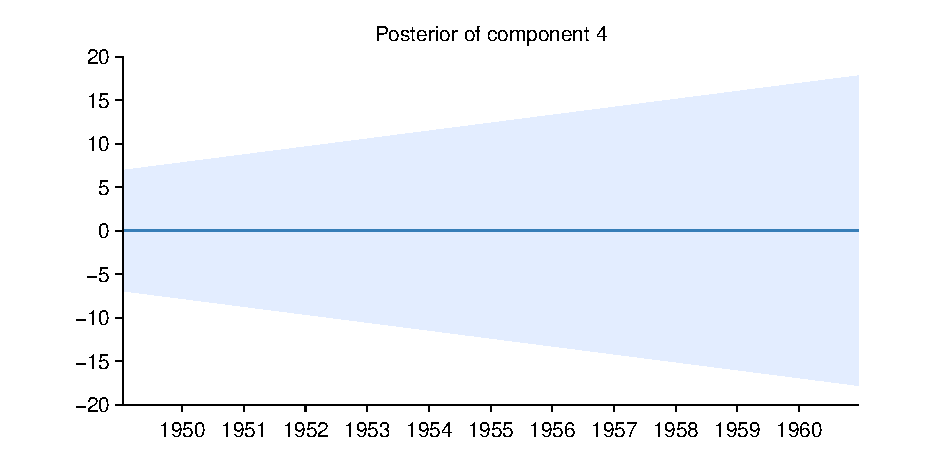
\includegraphics[width=0.5\textwidth]{figures/airline/01-airline_4.pdf}
      };
    \end{scope}
  \end{scope}
\end{tikzpicture}

%\end{center}
%
David Duvenaud, James Robert Lloyd, Roger Grosse, Joshua B. Tenenbaum, Zoubin Ghahramani
}
%\institute{
%\includegraphics[width=0.4\textwidth]{figures/spiral_main}
%\date{}


\begin{document}

\frame[plain] {
%\titlepage

\begin{center}

{ \color{darkblue} Structure Discovery in Nonparametric Regression through Compositional Kernel Search }


\begin{minipage}[t][6.8cm][t]{0.8\textwidth}
\begin{center}
\vspace{2.5cm}
  \begin{tikzpicture}[transform canvas={scale=0.9}] 
  \begin{scope}[yshift=0.2\textwidth]
    \begin{scope}[xshift=0cm]
      \node [mybox] (all) at (0, 0) {
        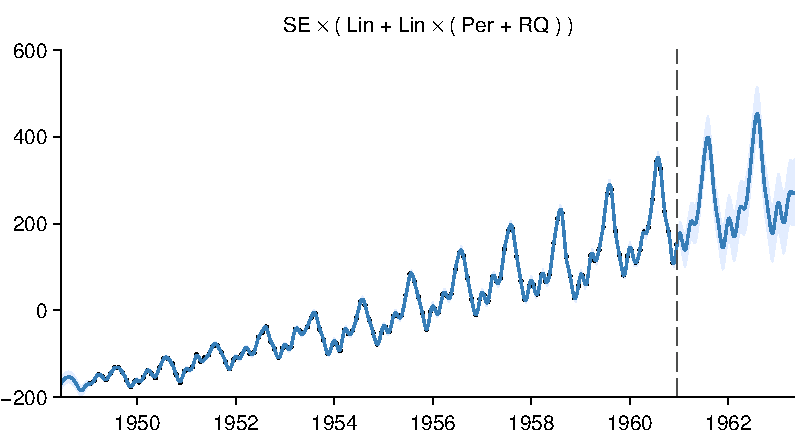
\includegraphics[trim=0 0 0 1.2cm, clip, width=0.8\textwidth, height=0.3\textwidth]{figures/01-airline-months_all.pdf}
      };
    \end{scope}
  \end{scope}
  \begin{scope}[yshift=0\textwidth]
    \begin{scope}[xshift=0cm]
    \end{scope}
  \end{scope}
  \begin{scope}[yshift=0.3\textwidth]
    \begin{scope}[xshift=4.12cm]
        \node [mybox, below of=all] (equals) at (0, 0) {\Huge{$=$}};
    \end{scope}
  \end{scope}
  \begin{scope}[yshift=-0.1\textwidth]
    \begin{scope}[xshift=-0.3\textwidth]
      \node [mybox] (all) at (0, 0) {
        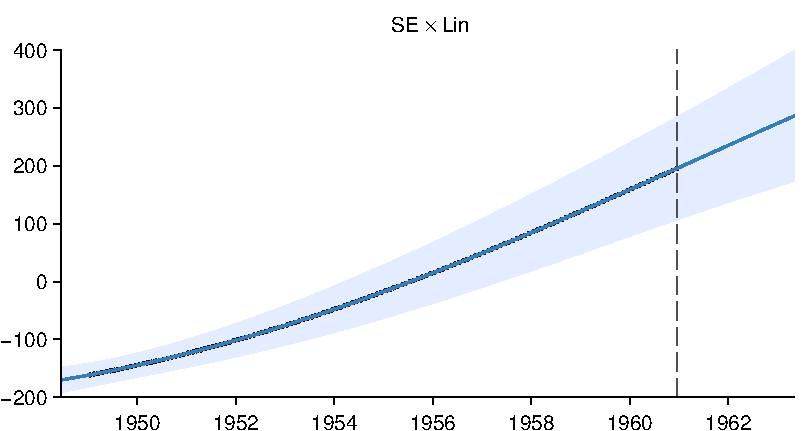
\includegraphics[trim=0 0 0 1.1cm, clip, width=0.5\textwidth]{figures/01-airline-months_1.pdf}
      };
    \end{scope}
    \begin{scope}[xshift=+0.3\textwidth]
      \node [mybox] (all) at (0, 0) {
        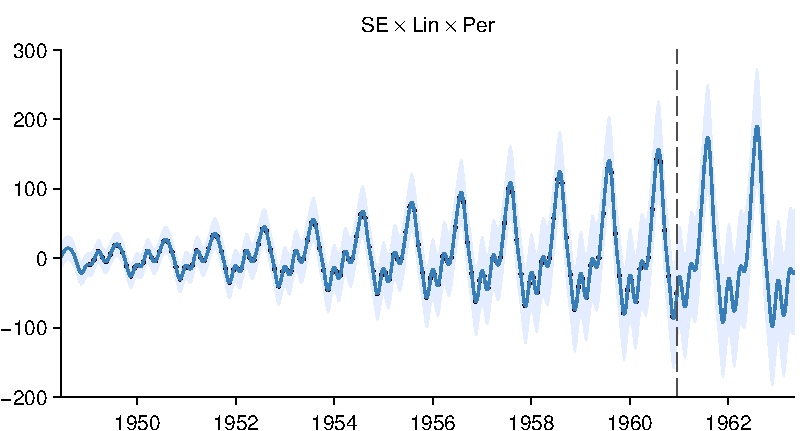
\includegraphics[trim=0 0 0 1.1cm, clip, width=0.5\textwidth]{figures/01-airline-months_2.pdf}
      };
    \end{scope}
  \end{scope}
  \begin{scope}[yshift=-0.15\textwidth]
    \begin{scope}[xshift=0cm]
        \node [mybox, below of=all] (equals) at (0, 0) {\Huge{+}};
    \end{scope}
  \end{scope}
  \begin{scope}[yshift=-0.35\textwidth]
    \begin{scope}[xshift=-0.3\textwidth]
      \node [mybox] (all) at (0, 0) {
        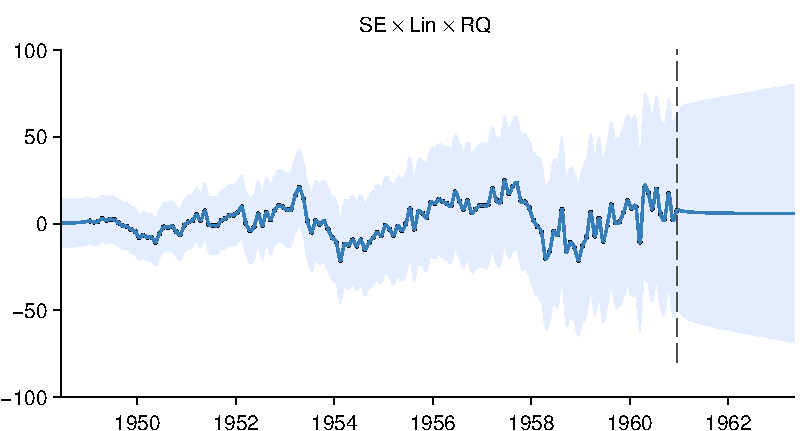
\includegraphics[trim=0 0 0 1.1cm, clip, width=0.5\textwidth]{figures/01-airline-months_3.pdf}
      };
    \end{scope}
    \begin{scope}[xshift=+0.3\textwidth]
      \node [mybox] (all) at (0, 0) {
        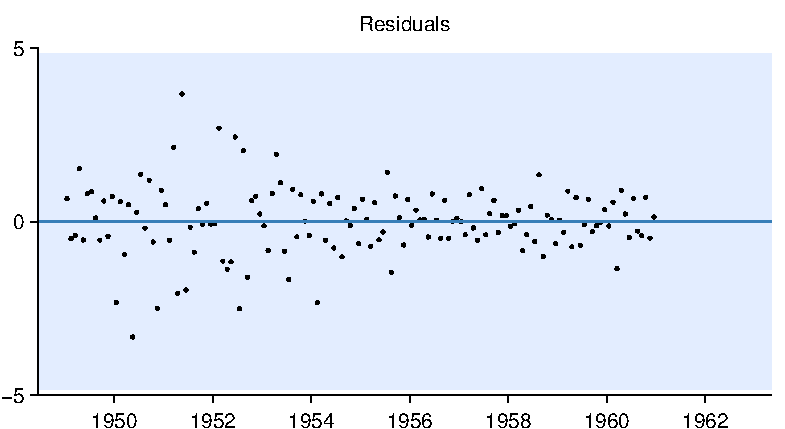
\includegraphics[trim=0 0 0 1.1cm, clip, width=0.5\textwidth]{figures/01-airline-months_resid.pdf}
      };
    \end{scope}
  \end{scope}
\end{tikzpicture}

\end{center}
\end{minipage}


David Duvenaud, James Robert Lloyd, Roger Grosse, \newline
Joshua B. Tenenbaum, Zoubin Ghahramani
\end{center}
}

\setbeamercolor{toc}{fg=black}

%\frame[plain]{
%\frametitle{GPs with complex kernels are powerful, interpretable models}
%\begin{center}
%  \begin{tikzpicture}[transform canvas={scale=0.9}] 
  \begin{scope}[yshift=0.2\textwidth]
    \begin{scope}[xshift=0cm]
      \node [mybox] (all) at (0, 0) {
        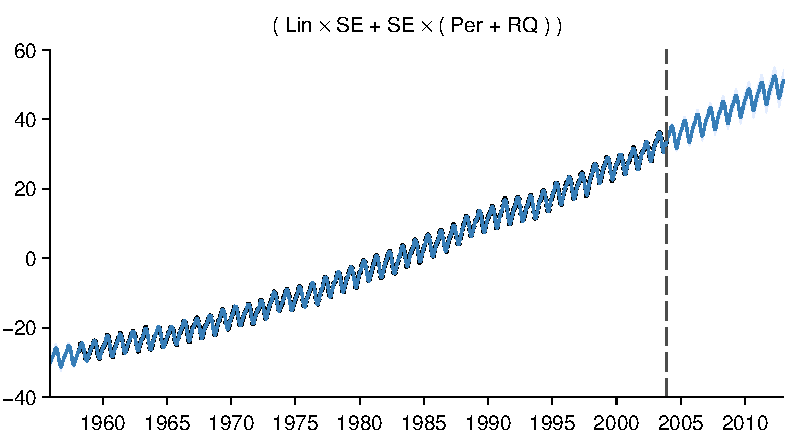
\includegraphics[width=0.8\textwidth, height=0.3\textwidth]{figures/03-mauna2003-s_all.pdf}
      };
    \end{scope}
  \end{scope}
  \begin{scope}[yshift=0\textwidth]
    \begin{scope}[xshift=0cm]
    \end{scope}
  \end{scope}
  \begin{scope}[yshift=0.27\textwidth]
    \begin{scope}[xshift=5cm]
        \node [mybox, below of=all] (equals) at (0, 0) {\Huge{$=$}};
    \end{scope}
  \end{scope}
  \begin{scope}[yshift=-0.1\textwidth]
    \begin{scope}[xshift=-0.3\textwidth]
      \node [mybox] (all) at (0, 0) {
        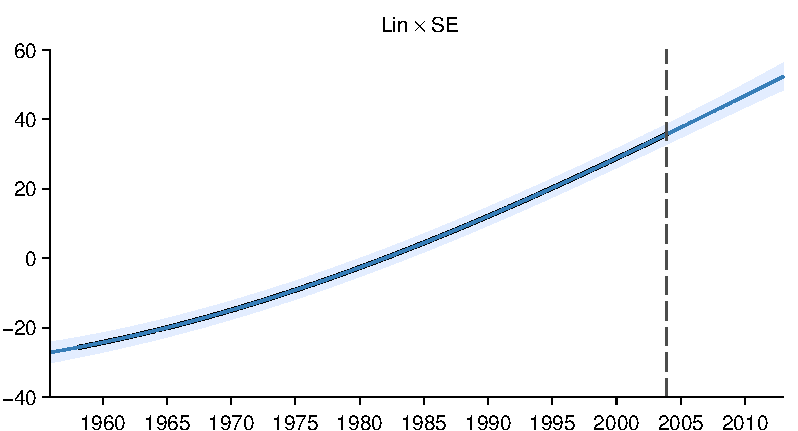
\includegraphics[width=0.5\textwidth]{figures/03-mauna2003-s_1.pdf}
      };
    \end{scope}
    \begin{scope}[xshift=+0.3\textwidth]
      \node [mybox] (all) at (0, 0) {
        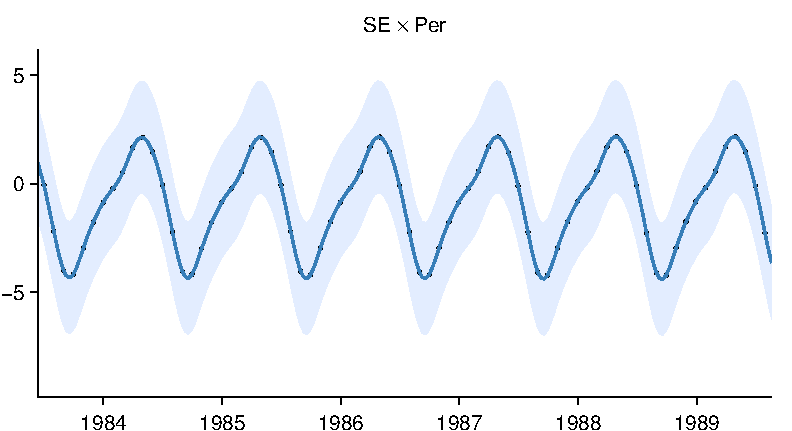
\includegraphics[width=0.5\textwidth]{figures/03-mauna2003-s_2_zoom.pdf}
      };
    \end{scope}
  \end{scope}
  \begin{scope}[yshift=-0.15\textwidth]
    \begin{scope}[xshift=0cm]
        \node [mybox, below of=all] (equals) at (0, 0) {\Huge{+}};
    \end{scope}
  \end{scope}
  \begin{scope}[yshift=-0.35\textwidth]
    \begin{scope}[xshift=-0.3\textwidth]
      \node [mybox] (all) at (0, 0) {
        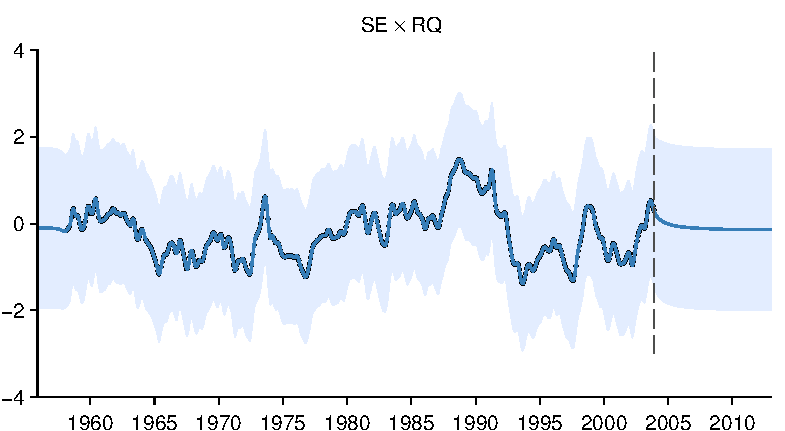
\includegraphics[width=0.5\textwidth]{figures/03-mauna2003-s_3.pdf}
      };
    \end{scope}
    \begin{scope}[xshift=+0.3\textwidth]
      \node [mybox] (all) at (0, 0) {
        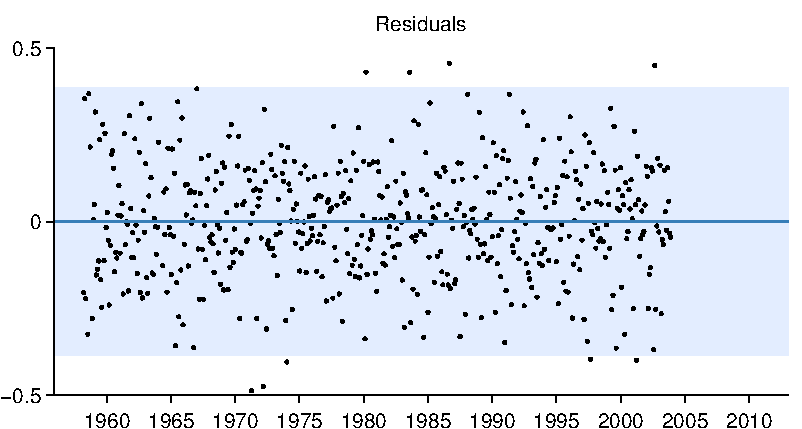
\includegraphics[width=0.5\textwidth]{figures/03-mauna2003-s_resid.pdf}
      };
    \end{scope}
  \end{scope}
\end{tikzpicture}

%\end{center}
%}


\frame[plain]{
%\frametitle{Simple kernels $\to$ simple structure}
\frametitle{Kernel Choice is Important}
%\begin{itemize} 
%	\item Kernel determines almost all the properties of a \gp{} model.
%	\item Many different kinds, with very different properties:
%\end{itemize}
\newcommand{\fhbig}{1.6cm}
\newcommand{\fwbig}{1.8cm}
\newcommand{\kernpic}[1]{\includegraphics[height=\fhbig,width=\fwbig]{figures/structure_examples/#1}}
\newcommand{\kernpicr}[1]{\rotatebox{90}{\includegraphics[height=\fwbig,width=\fhbig]{figures/structure_examples/#1}}}
\newcommand{\addkernpic}[1]{{\includegraphics[height=\fhbig,width=\fwbig]{figures/additive_multi_d/#1}}}
\newcommand{\largeplus}{\tabbox{{\Large+}}}
\newcommand{\largeeq}{\tabbox{{\Large=}}}
\newcommand{\largetimes}{\tabbox{{\Large$\times$}}}
\begin{figure}[ht]
\centering
\renewcommand{\tabularxcolumn}[1]{>{\arraybackslash}m{#1}}
%\begin{tabular}{m{\fwbig}m{0.01\textwidth}m{\fwbig}m{0.01\textwidth}m{\fwbig}m{\fwbig}m{\fwbig}}
%\begin{tabular}{C{\fwbig}C{\fwbig}C{\fwbig}C{\fwbig}}%{m{\fwbig}m{\fwbig}m{\fwbig}}
\begin{tabularx}{\columnwidth}{XXcXX}
%Composite & Draws from \gp{} & \gp{} posterior \\ \toprule
  \kernpic{se_kernel} & \kernpic{se_kernel_draws} & \phantom{mm}
& \kernpic{per_kernel} & \kernpic{per_kernel_draws_s2}
\\
  {\small Squared-exp (\kSE)} & {\small local \newline variation} & \phantom{mm}
& {\small Periodic (\kPer)} & {\small repeating structure}
\\ \\ \\
  \kernpic{lin_kernel} & \kernpic{lin_kernel_draws} & \phantom{mm}
& \kernpic{rq_kernel} & \kernpic{rq_kernel_draws}
\\
  {\small Linear (\kLin)} & {\small linear \newline functions}  & \phantom{mm}
& {\small Rational-quadratic(\kRQ)} & {\small multi-scale variation}
\end{tabularx}
\end{figure}


}



\frame[plain]{
\frametitle{Identifying structure is crucial for extrapolation}
%\begin{itemize} 
%	\item SE kernel $\rightarrow$ basic smoothing.
%	\item Richer kernels means richer structure can be captured.
%\end{itemize}
%\begin{center}
%  \begin{tikzpicture}%[transform canvas={scale = 0.9}]
  \begin{scope}[yshift=0\textwidth]
    \begin{scope}[xshift=-0.3\textwidth]
      \node [mybox] at (0, 0) {
        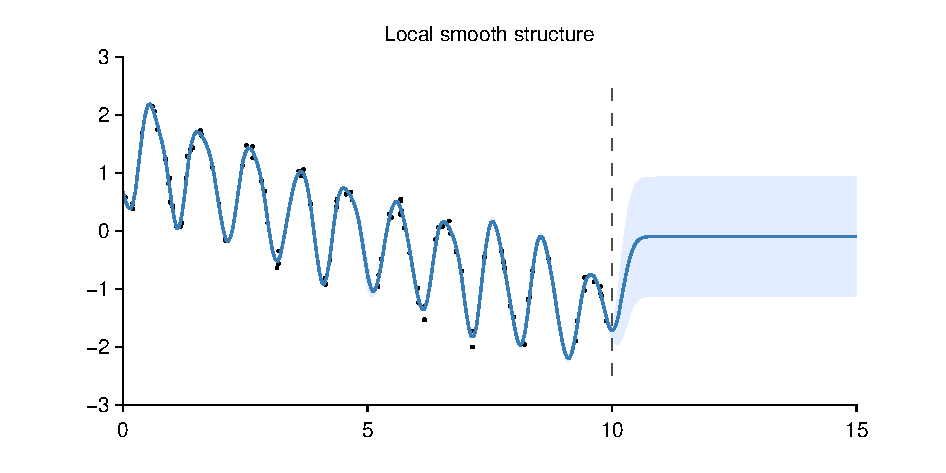
\includegraphics[width=0.5\textwidth]{figures/synth_extrap_bad.pdf}
      };
    \end{scope}
    \begin{scope}[xshift=+0.2\textwidth]
      \node [mybox] at (0, 0) {
        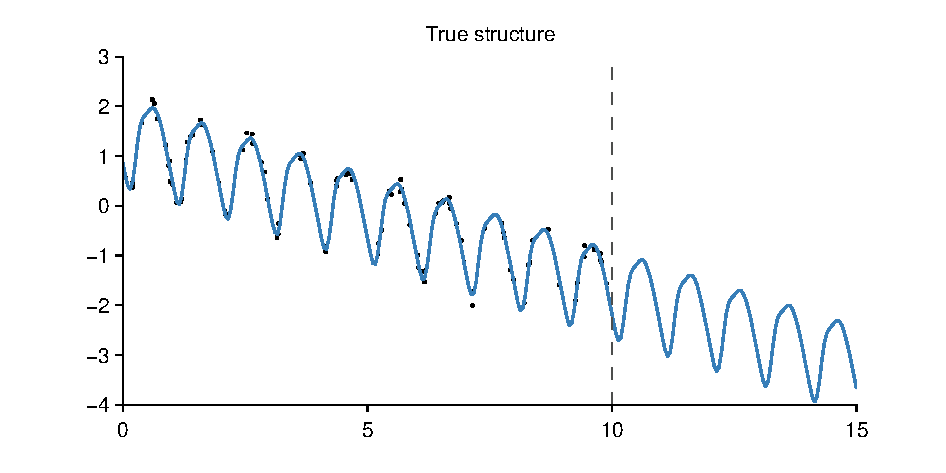
\includegraphics[width=0.5\textwidth]{figures/synth_extrap_good.pdf}
      };
    \end{scope}
  \end{scope}
\end{tikzpicture}


%\end{center}
\begin{center}
\begin{tabular}{cc}
local smoothing \\
%\hspace{-1.5cm}
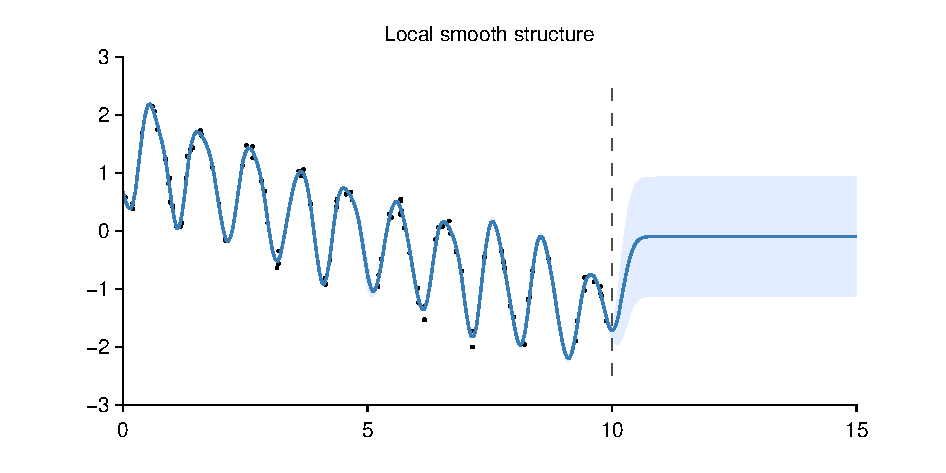
\includegraphics[trim=0 0 0 1.2cm, clip, width=0.99\textwidth, height=3cm]{figures/synth_extrap_bad.pdf}
\\
\phantom{structured model} \\
%\hspace{-3cm}
\phantom{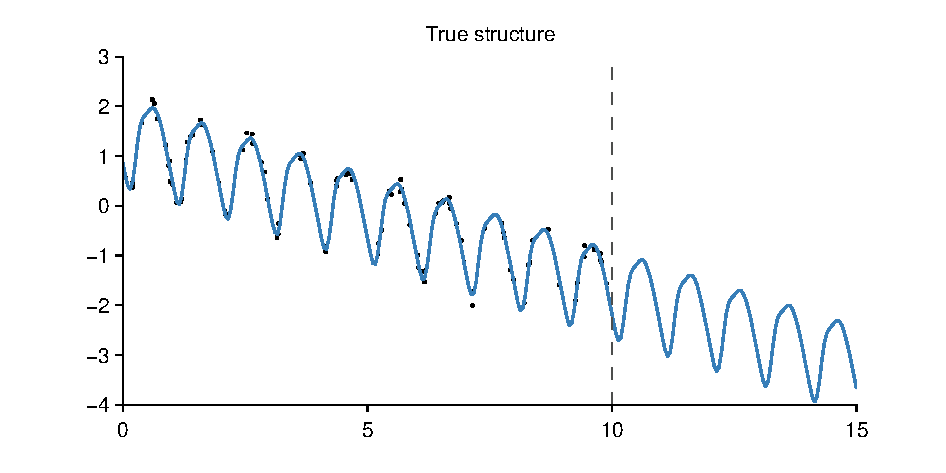
\includegraphics[trim=0 0 0 1.2cm, clip, width=0.99\textwidth, height=3cm]{figures/synth_extrap_good.pdf}}
%  \begin{tikzpicture}%[transform canvas={scale = 0.9}]
  \begin{scope}[yshift=0\textwidth]
    \begin{scope}[xshift=-0.3\textwidth]
      \node [mybox] at (0, 0) {
        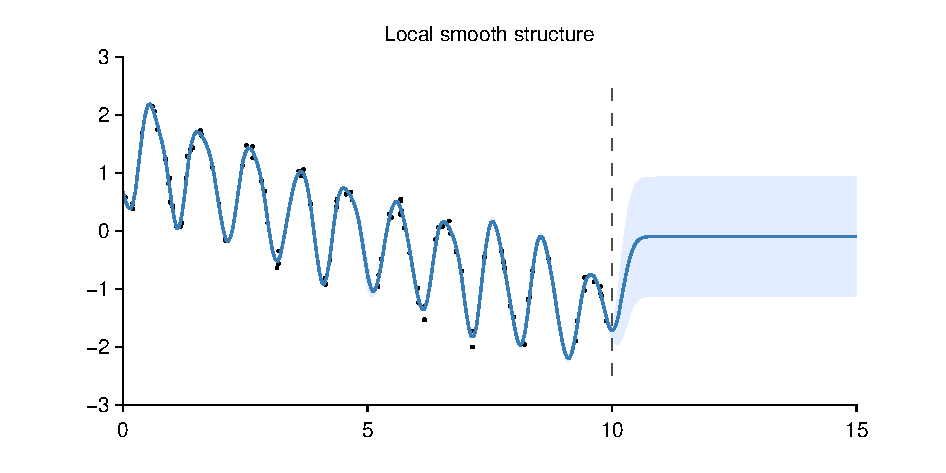
\includegraphics[width=0.5\textwidth]{figures/synth_extrap_bad.pdf}
      };
    \end{scope}
    \begin{scope}[xshift=+0.2\textwidth]
      \node [mybox] at (0, 0) {
        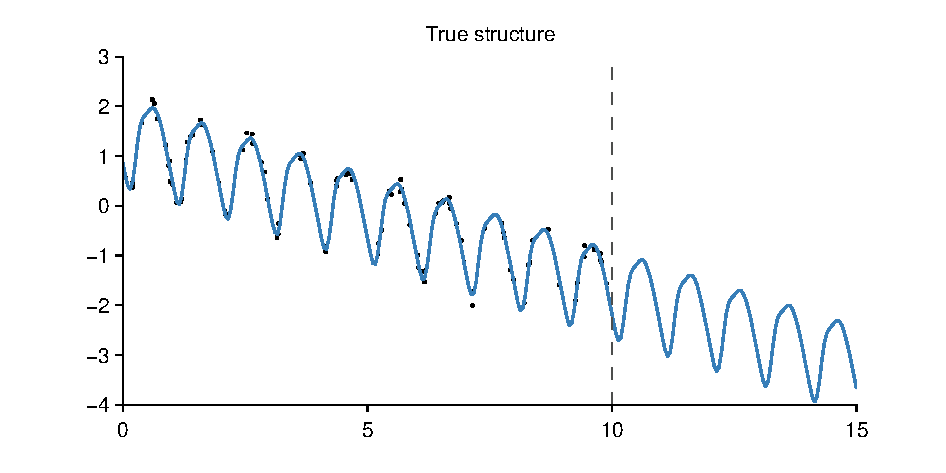
\includegraphics[width=0.5\textwidth]{figures/synth_extrap_good.pdf}
      };
    \end{scope}
  \end{scope}
\end{tikzpicture}


\end{tabular}
\end{center}
}


\frame[plain]{
%\frametitle{Composite kernels $\to$ richer structure}
\frametitle{Kernels can be Composed}
%\begin{itemize} 
%	\item Two main operations: adding, multiplying
	\newcommand{\fhbig}{1.6cm}
\newcommand{\fwbig}{1.8cm}
\newcommand{\kernpic}[1]{\includegraphics[height=\fhbig,width=\fwbig]{figures/structure_examples/#1}}
\newcommand{\kernpicr}[1]{\rotatebox{90}{\includegraphics[height=\fwbig,width=\fhbig]{figures/structure_examples/#1}}}
\newcommand{\addkernpic}[1]{{\includegraphics[height=\fhbig,width=\fwbig]{figures/additive_multi_d/#1}}}
\newcommand{\largeplus}{\tabbox{{\Large+}}}
\newcommand{\largeeq}{\tabbox{{\Large=}}}
\newcommand{\largetimes}{\tabbox{{\Large$\times$}}}
\begin{figure}[ht]
\centering
\renewcommand{\tabularxcolumn}[1]{>{\arraybackslash}m{#1}}
%\begin{tabular}{m{\fwbig}m{0.01\textwidth}m{\fwbig}m{0.01\textwidth}m{\fwbig}m{\fwbig}m{\fwbig}}
%\begin{tabular}{C{\fwbig}C{\fwbig}C{\fwbig}C{\fwbig}}%{m{\fwbig}m{\fwbig}m{\fwbig}}
\begin{tabularx}{\columnwidth}{XXcXX}
  \kernpic{lin_times_lin} & \kernpic{lin_times_lin_draws} & \phantom{mm}
& \kernpic{longse_times_per} & \kernpic{longse_times_per_draws_s1}
\\
  {\small $\kLin \times \kLin$} & {\small quadratic functions} & \phantom{mm}
& {\small $\kSE \times \kPer$} & {\small locally \newline periodic}
\\ \\ \\
%\midrule 
  \kernpic{lin_plus_per} & \kernpic{lin_plus_per_draws} & \phantom{mm} 
& \kernpic{se_plus_per} & \kernpic{se_plus_per_draws_s7}
\\
  {\small $\kLin + \kPer$} & {\small periodic with trend} & \phantom{mm}
& {\small $\kSE + \kPer$ } & {\small periodic with noise}
\end{tabularx}
\end{figure}


%\end{itemize}
}


\frame[plain]{
\frametitle{Identifying structure is crucial for extrapolation}
%\begin{itemize} 
%	\item SE kernel $\rightarrow$ basic smoothing.
%	\item Richer kernels means richer structure can be captured.
%\end{itemize}
%\begin{center}
%  \begin{tikzpicture}%[transform canvas={scale = 0.9}]
  \begin{scope}[yshift=0\textwidth]
    \begin{scope}[xshift=-0.3\textwidth]
      \node [mybox] at (0, 0) {
        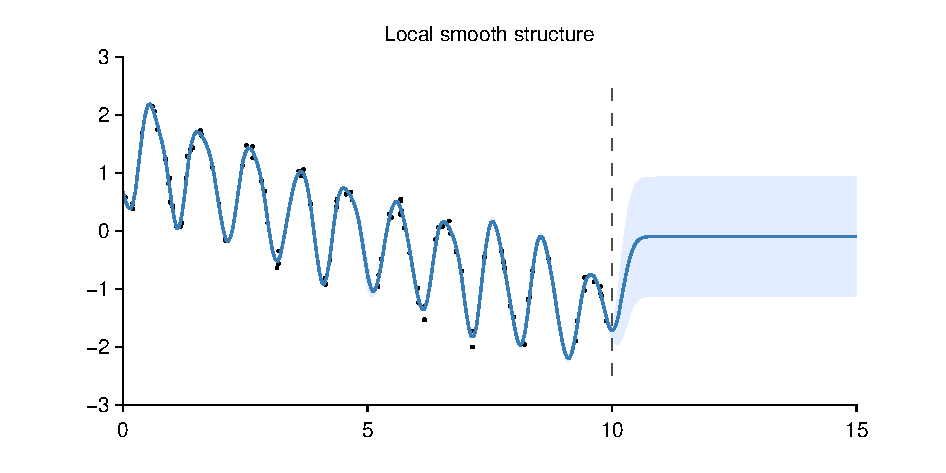
\includegraphics[width=0.5\textwidth]{figures/synth_extrap_bad.pdf}
      };
    \end{scope}
    \begin{scope}[xshift=+0.2\textwidth]
      \node [mybox] at (0, 0) {
        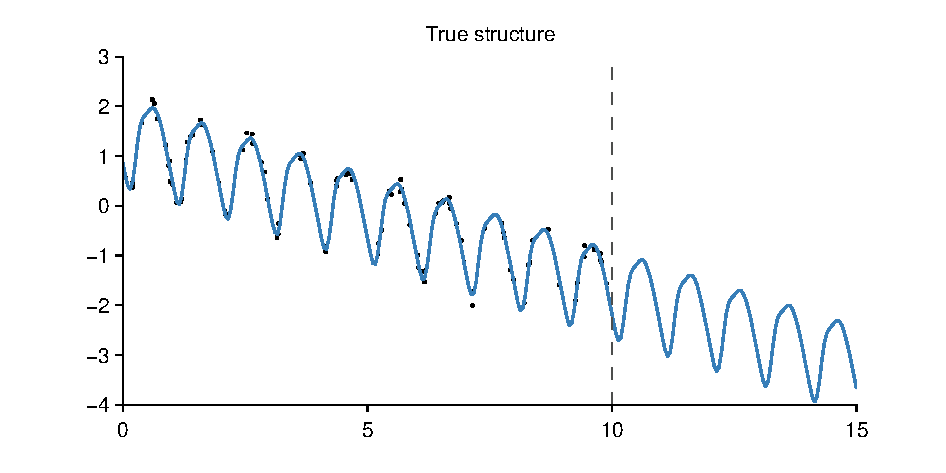
\includegraphics[width=0.5\textwidth]{figures/synth_extrap_good.pdf}
      };
    \end{scope}
  \end{scope}
\end{tikzpicture}


%\end{center}
\begin{center}
\begin{tabular}{cc}
local smoothing \\
%\hspace{-1.5cm}
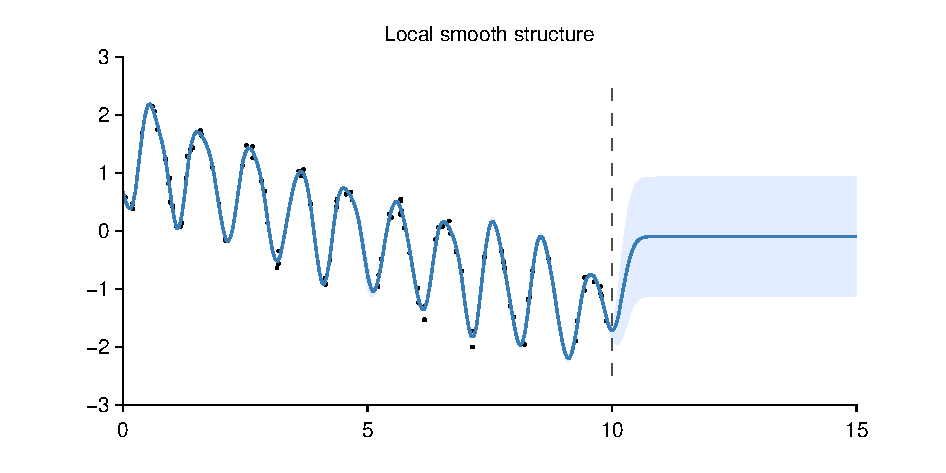
\includegraphics[trim=0 0 0 1.2cm, clip, width=0.99\textwidth, height=3cm]{figures/synth_extrap_bad.pdf}
\\
structured model \\
%\hspace{-3cm}
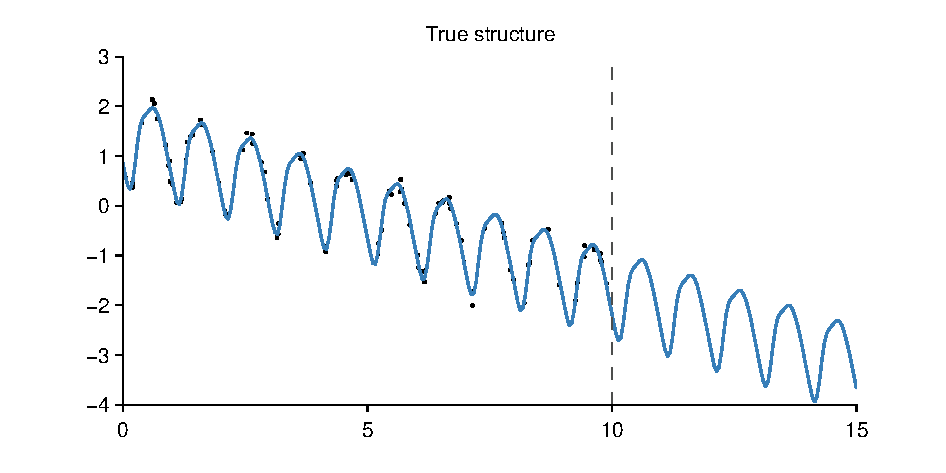
\includegraphics[trim=0 0 0 1.2cm, clip, width=0.99\textwidth, height=3cm]{figures/synth_extrap_good.pdf}
%  \begin{tikzpicture}%[transform canvas={scale = 0.9}]
  \begin{scope}[yshift=0\textwidth]
    \begin{scope}[xshift=-0.3\textwidth]
      \node [mybox] at (0, 0) {
        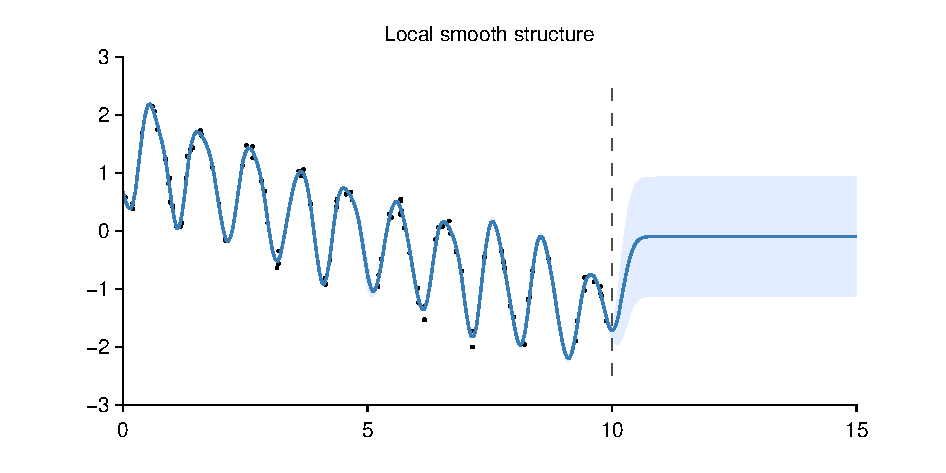
\includegraphics[width=0.5\textwidth]{figures/synth_extrap_bad.pdf}
      };
    \end{scope}
    \begin{scope}[xshift=+0.2\textwidth]
      \node [mybox] at (0, 0) {
        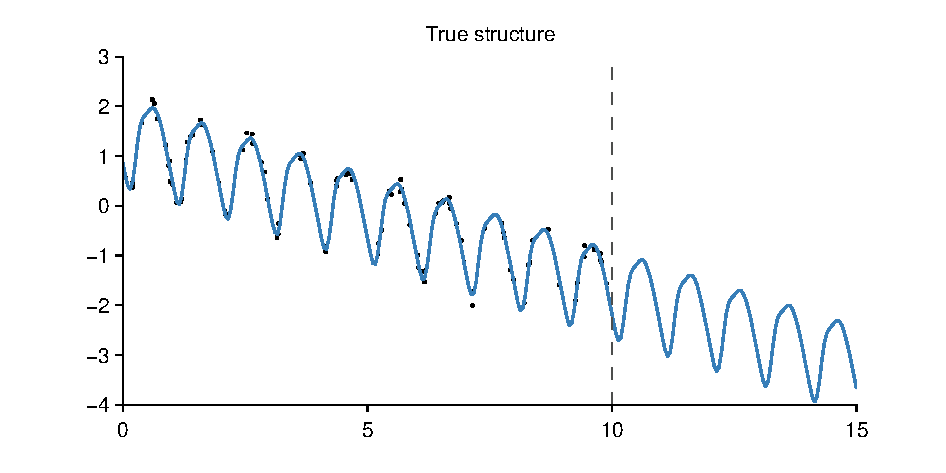
\includegraphics[width=0.5\textwidth]{figures/synth_extrap_good.pdf}
      };
    \end{scope}
  \end{scope}
\end{tikzpicture}


\end{tabular}
\end{center}
}


\frame[plain]{
\frametitle{Compositional Structure Search}
\begin{itemize}
	\item We define simple grammar over kernels:
	\begin{itemize}
		\item $ K \rightarrow K + K$ 
		\item $ K \rightarrow K \times K$ 
		%\item $ K \rightarrow \{ \SE, \RQ, \Lin, \Per \}$
		\item $K \rightarrow \SE\ |\ \RQ\ |\ \Lin\ |\ \Per $
	\end{itemize}
	\item Can automatically search open-ended space of kernels by applying production rules, then checking model fit (approximate marginal likelihood).
\end{itemize}
}


%\frame[plain]{
%\frametitle{Kernels can be composed}
%\begin{itemize} 
%	\item Can be composed across multiple dimensions
%	\newcommand{\fhbig}{1.6cm}
\newcommand{\fwbig}{1.8cm}
\newcommand{\kernpic}[1]{\includegraphics[height=\fhbig,width=\fwbig]{figures/structure_examples/#1}}
\newcommand{\kernpicr}[1]{\rotatebox{90}{\includegraphics[height=\fwbig,width=\fhbig]{figures/structure_examples/#1}}}
\newcommand{\addkernpic}[1]{{\includegraphics[height=\fhbig,width=\fwbig]{figures/additive_multi_d/#1}}}
\newcommand{\largeplus}{\tabbox{{\Large+}}}
\newcommand{\largeeq}{\tabbox{{\Large=}}}
\newcommand{\largetimes}{\tabbox{{\Large$\times$}}}
\begin{figure}[ht]
\centering
\renewcommand{\tabularxcolumn}[1]{>{\arraybackslash}m{#1}}
%\begin{tabular}{m{\fwbig}m{0.01\textwidth}m{\fwbig}m{0.01\textwidth}m{\fwbig}m{\fwbig}m{\fwbig}}
%\begin{tabular}{C{\fwbig}C{\fwbig}C{\fwbig}C{\fwbig}}%{m{\fwbig}m{\fwbig}m{\fwbig}}
\begin{tabularx}{\columnwidth}{XXXX}
  \kernpic{se_times_lin} & \kernpic{se_times_lin_draws_s2}
& \kernpic{lin_times_per} & \kernpic{lin_times_per_draws_s2}
\\
  {\small $\kLin \times \kSE$} & {\small increasing variation}
& {\small $\kLin \times \kPer$} & {\small growing amplitude}
\\
  \addkernpic{additive_kernel} & \addkernpic{additive_kernel_draw_sum}
& \addkernpic{sqexp_kernel}  & \addkernpic{sqexp_draw}
\\
  {\small $\kSE_1 + \kSE_2$} & {\small $f_1(x_1)$ $+ f_2(x_2)$}
& {\small $\kSE_1 \times \kSE_2$} & {\small $f(x_1, x_2)$}
\end{tabularx}
\end{figure}


%\end{itemize}
%}

\tikzset{hide on/.code={\only<#1>{\color{white}}}}

\frame[plain]{
\frametitle{Compositional Structure Search}
\hspace{-1.2cm}
\only<1>{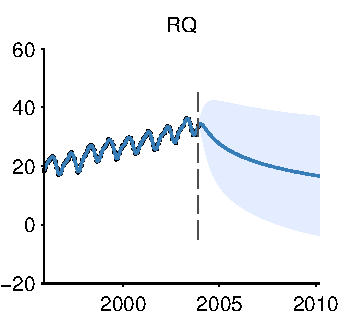
\includegraphics[width=0.4\textwidth]{figures/11-Feb-v4-03-mauna2003-s_max_level_0/03-mauna2003-s_all_small.pdf}}
\only<2>{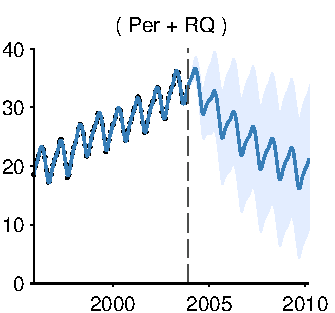
\includegraphics[width=0.4\textwidth]{figures/11-Feb-v4-03-mauna2003-s_max_level_1/03-mauna2003-s_all_small.pdf}}
\only<3>{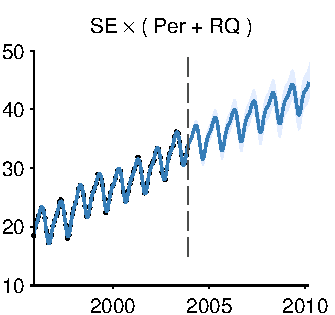
\includegraphics[width=0.4\textwidth]{figures/11-Feb-v4-03-mauna2003-s_max_level_2/03-mauna2003-s_all_small.pdf}}
\only<4>{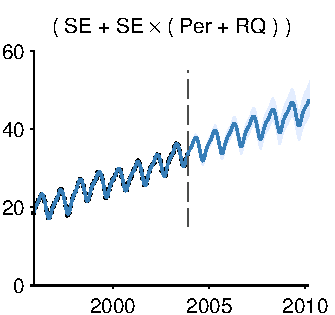
\includegraphics[width=0.4\textwidth]{figures/11-Feb-v4-03-mauna2003-s_max_level_3/03-mauna2003-s_all_small.pdf}}

\vspace{-3.5cm}
\begin{minipage}[t][14cm][t]{1.14\linewidth}
\begin{flushleft}
\hspace{5.5cm}
\vspace{-8cm}
\makebox[\textwidth][c]{
\raisebox{10cm}{
\vspace{-8cm}
\begin{tikzpicture}
[sibling distance=0.18\columnwidth,-,thick, level distance=0.13\columnwidth]
%\footnotesize
\node[shape=rectangle,draw,thick] {Start}
%\pause
  child {node {$\SE$}}
%  fill=camlightblue!30
  child {node[shape=rectangle,draw,thick] {$\RQ$}
    [sibling distance=0.16\columnwidth]
%    {\visible<2->{ child {node {\ldots}}}}
    child [hide on=-1] {node {$\SE$ + \RQ}}
    child [hide on=-1] {node {\ldots}}
    child [hide on=-1] {node[shape=rectangle,draw,thick] {$\Per + \RQ$}
      [sibling distance=0.23\columnwidth]
      child [hide on=-2] {node {$\SE + \Per + \RQ$}}
      child [hide on=-2] {node {\ldots}}
      child [hide on=-2] {node[shape=rectangle,draw,thick] {$\SE \times (\Per + \RQ)$}
        [sibling distance=0.14\columnwidth]
        child [hide on=-3] {node {\ldots}}
        child [hide on=-3] {node {\ldots}}
        child [hide on=-3] {node {\ldots}}
      }
      child [hide on=-2] {node {\ldots}}
    }
    %child {node {$\RQ \times \SE$}}
    child [hide on=-1] {node {\ldots}}
    child [hide on=-1] {node {$\Per \times \RQ$}}
  }
  child {node {$\Lin$}}
  child {node {$\Per$}}
  ;
\end{tikzpicture}}
}\end{flushleft}
\end{minipage}
\only<4>{}
}

\frame[plain]{
\frametitle{Decomposing the posterior}
\begin{center}
  \begin{tikzpicture}[transform canvas={scale=0.9}] 
  \begin{scope}[yshift=0.2\textwidth]
    \begin{scope}[xshift=0cm]
      \node [mybox] (all) at (0, 0) {
	  \begin{tabular}{c}
	  {\small $\Lin \times \SE + \SE \times ( \Per + \RQ)$ } \\	  
        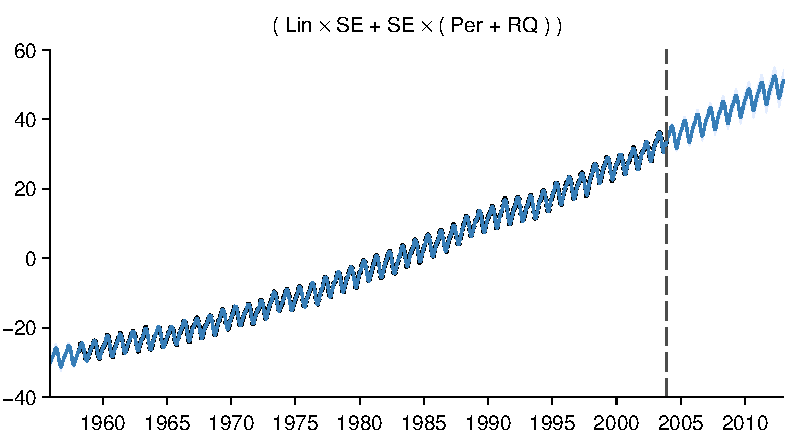
\includegraphics[trim=0 0 0 1.2cm, clip, width=0.8\textwidth, height=0.28\textwidth]{figures/03-mauna2003-s_all.pdf}
		\end{tabular}
      };
    \end{scope}
  \end{scope}
  \begin{scope}[yshift=0.3\textwidth]
    \begin{scope}[xshift=4.8cm]
        \node [mybox, below of=all] (equals) at (0, 0) {\Huge{$=$}};
    \end{scope}
  \end{scope}
  \begin{scope}[yshift=-0.11\textwidth]
    \begin{scope}[xshift=-0.3\textwidth]
      \node [mybox] (all) at (0, 0) {
	  	  \begin{tabular}{c}
	  {\small $\Lin \times \SE$ } \\	 
        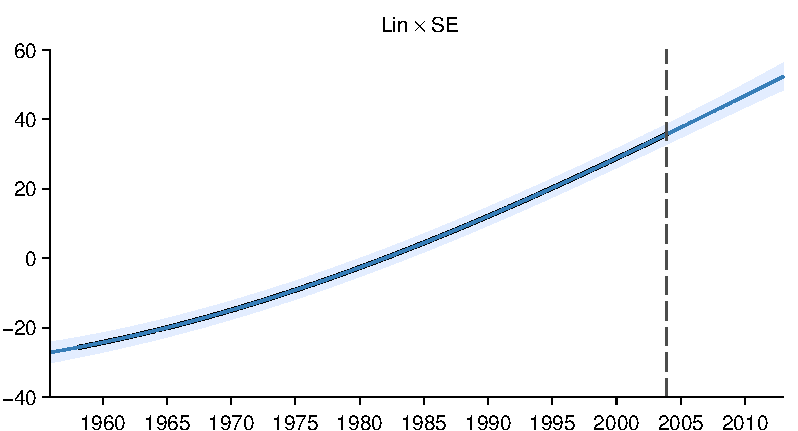
\includegraphics[trim=0 0 0 1.1cm, clip, width=0.5\textwidth, height=2.2cm]{figures/03-mauna2003-s_1.pdf}
		\end{tabular}
      };
    \end{scope}
    \begin{scope}[xshift=+0.3\textwidth]
      \node [mybox] (all) at (0, 0) {
	  	  \begin{tabular}{c}
	   {\small $\SE \times \Per$ } \\	 
        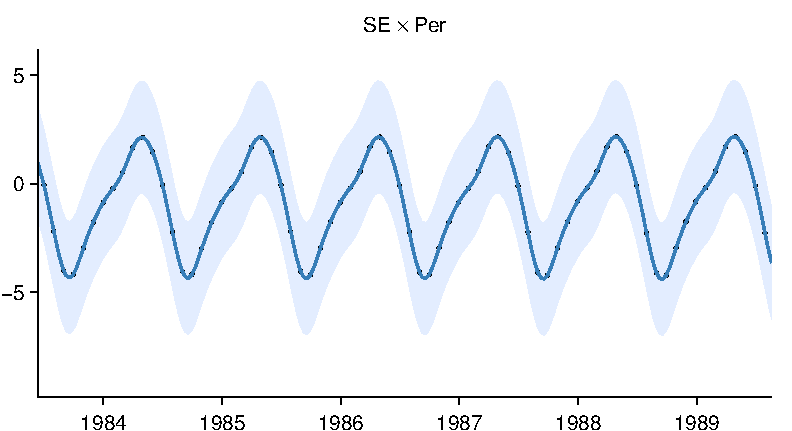
\includegraphics[trim=0 0 0 1.1cm, clip, width=0.5\textwidth, height=2.2cm]{figures/03-mauna2003-s_2_zoom.pdf}
		\end{tabular}
      };
    \end{scope}
  \end{scope}
  \begin{scope}[yshift=-0.16\textwidth]
    \begin{scope}[xshift=0cm]
        \node [mybox, below of=all] (equals) at (0, 0) {\Huge{+}};
    \end{scope}
  \end{scope}
  \begin{scope}[yshift=-0.38\textwidth]
    \begin{scope}[xshift=-0.3\textwidth]
      \node [mybox] (all) at (0, 0) {
	  	  \begin{tabular}{c}
	  {\small $\SE \times \RQ$ } \\	 
        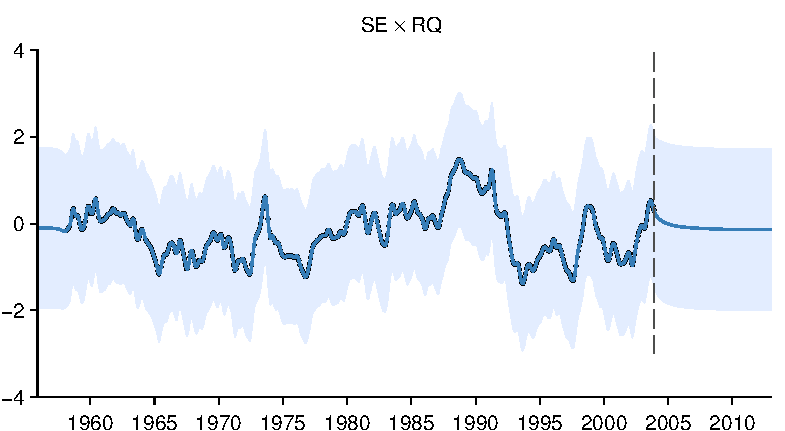
\includegraphics[trim=0 0 0 1.1cm, clip, width=0.5\textwidth, height=2.2cm]{figures/03-mauna2003-s_3.pdf}
		\end{tabular}
      };
    \end{scope}
    \begin{scope}[xshift=+0.3\textwidth]
      \node [mybox] (all) at (0, 0) {
	  	  \begin{tabular}{c}
	  {\small Residuals } \\	 
        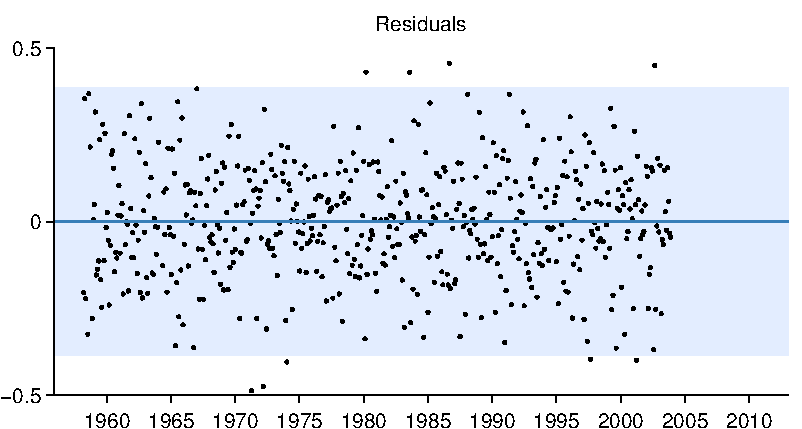
\includegraphics[trim=0 0 0 1.1cm, clip, width=0.5\textwidth, height=2.2cm]{figures/03-mauna2003-s_resid.pdf}
		\end{tabular}
      };
    \end{scope}
  \end{scope}
\end{tikzpicture}

\end{center}
}



%\frame[plain]{
%\frametitle{Example: Airline passengers}
%\begin{center}
%  \begin{tikzpicture}[transform canvas={scale=0.9}] 
  \begin{scope}[yshift=0.2\textwidth]
    \begin{scope}[xshift=0cm]
      \node  (all) at (0, 0) {
	  \begin{tabular}{c}
	  {\small $\SE \times ( \Lin + \Lin \times ( \Per + \RQ))$ } \\	  
        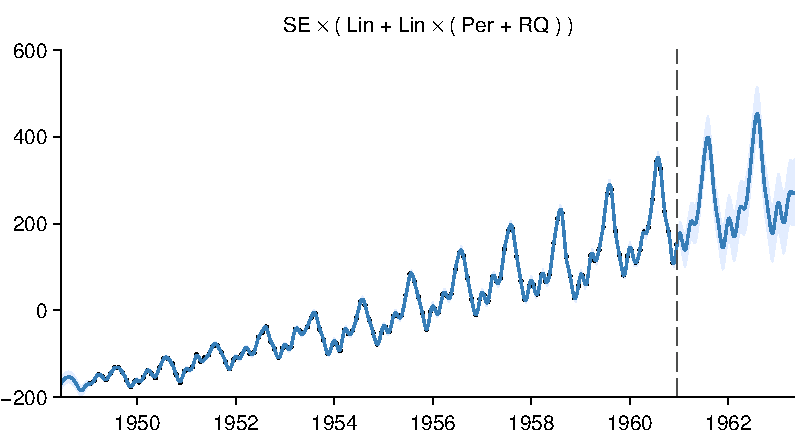
\includegraphics[trim=0 0 0 1.2cm, clip, width=0.8\textwidth, height=0.28\textwidth]{figures/01-airline-months_all.pdf}
		\end{tabular}
      };
    \end{scope}
  \end{scope}
  \begin{scope}[yshift=0.3\textwidth]
    \begin{scope}[xshift=4.8cm]
        \node [mybox, below of=all] (equals) at (0, 0) {\Huge{$=$}};
    \end{scope}
  \end{scope}
  \begin{scope}[yshift=-0.11\textwidth]
    \begin{scope}[xshift=-0.3\textwidth]
      \node [mybox] (all) at (0, 0) {
	  	  \begin{tabular}{c}
	  {\small $\SE \times \Lin$ } \\	 
        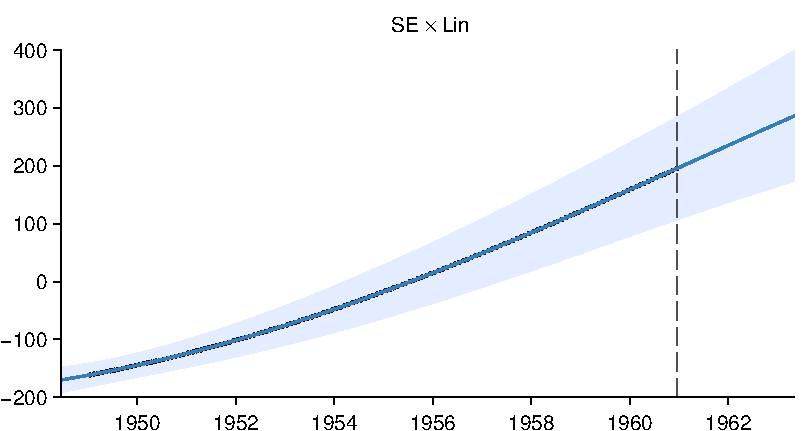
\includegraphics[trim=0 0 0 1.1cm, clip, width=0.5\textwidth, height=2.2cm]{figures/01-airline-months_1.pdf}
		\end{tabular}
      };
    \end{scope}
    \begin{scope}[xshift=+0.3\textwidth]
      \node [mybox] (all) at (0, 0) {
	  	  \begin{tabular}{c}
	   {\small $\SE \times \Lin \times \Per$ } \\	 
        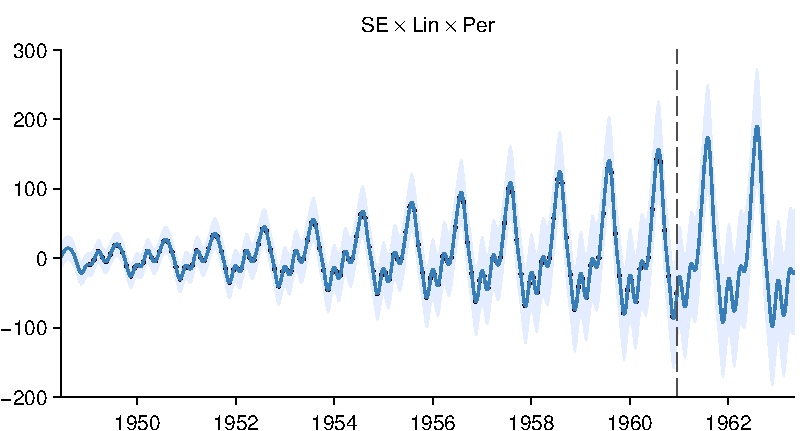
\includegraphics[trim=0 0 0 1.1cm, clip, width=0.5\textwidth, height=2.2cm]{figures/01-airline-months_2.pdf}
		\end{tabular}
      };
    \end{scope}
  \end{scope}
  \begin{scope}[yshift=-0.16\textwidth]
    \begin{scope}[xshift=0cm]
        \node [mybox, below of=all] (equals) at (0, 0) {\Huge{+}};
    \end{scope}
  \end{scope}
  \begin{scope}[yshift=-0.38\textwidth]
    \begin{scope}[xshift=-0.3\textwidth]
      \node [mybox] (all) at (0, 0) {
	  	  \begin{tabular}{c}
	  {\small $\SE \times \Lin \times \RQ$ } \\	 
        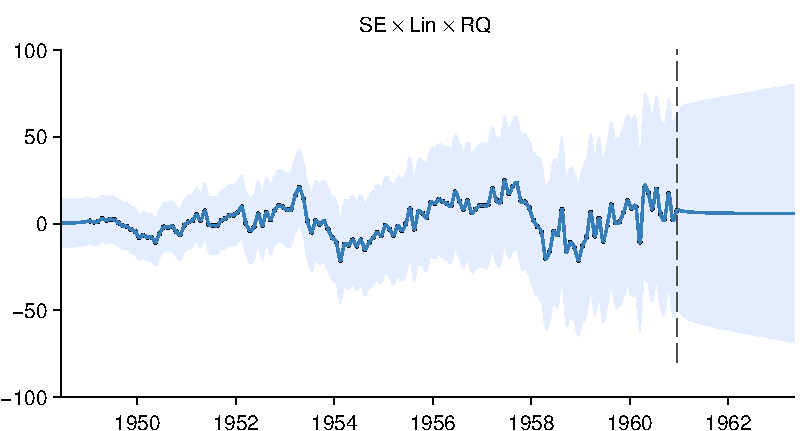
\includegraphics[trim=0 0 0 1.1cm, clip, width=0.5\textwidth, height=2.2cm]{figures/01-airline-months_3.pdf}
		\end{tabular}
      };
    \end{scope}
    \begin{scope}[xshift=+0.3\textwidth]
      \node [mybox] (all) at (0, 0) {
	  	  \begin{tabular}{c}
	  {\small Residuals } \\	 
        \includegraphics[trim=0 0 0 1.1cm, clip, width=0.5\textwidth, height=2.2cm]{figures/01-airline-months_resid.pdf}
		\end{tabular}
      };
    \end{scope}
  \end{scope}
\end{tikzpicture}

%\end{center}
%}

\frame[plain]{
\frametitle{Example: Radio critical frequency }
\begin{center}
  \begin{tikzpicture}[transform canvas={scale=0.9}] 
  \begin{scope}[yshift=0.2\textwidth]
    \begin{scope}[xshift=0cm]
      \node [mybox] (all) at (0, 0) {
	  \begin{tabular}{c}
	  {\small $( \SE + \RQ ) \times ( \Per + \CS)$  } \\	  
        \includegraphics[trim=0 0 0 1.2cm, clip, width=0.8\textwidth, height=0.28\textwidth]{figures/radio/all.pdf}
		\end{tabular}
      };
    \end{scope}
  \end{scope}
  \begin{scope}[yshift=0.3\textwidth]
    \begin{scope}[xshift=4.8cm]
        \node [mybox, below of=all] (equals) at (0, 0) {\Huge{$=$}};
    \end{scope}
  \end{scope}
  \begin{scope}[yshift=-0.11\textwidth]
    \begin{scope}[xshift=-0.3\textwidth]
      \node [mybox] (all) at (0, 0) {
	  	  \begin{tabular}{c}
	  {\small $\SE$ } \\	 
        \includegraphics[trim=0 0 0 1.1cm, clip, width=0.5\textwidth, height=2.2cm]{figures/radio/3.pdf}
		\end{tabular}
      };
    \end{scope}
    \begin{scope}[xshift=+0.3\textwidth]
      \node [mybox] (all) at (0, 0) {
	  	  \begin{tabular}{c}
	   {\small $\Per \times \RQ$ } \\	 
        \includegraphics[trim=0 0 0 1.1cm, clip, width=0.5\textwidth, height=2.2cm]{figures/radio/4.pdf}
		\end{tabular}
      };
    \end{scope}
  \end{scope}
  \begin{scope}[yshift=-0.16\textwidth]
    \begin{scope}[xshift=0cm]
        \node [mybox, below of=all] (equals) at (0, 0) {\Huge{+}};
    \end{scope}
  \end{scope}
  \begin{scope}[yshift=-0.38\textwidth]
    \begin{scope}[xshift=-0.3\textwidth]
      \node [mybox] (all) at (0, 0) {
	  	  \begin{tabular}{c}
	  {\small $\Per \times \SE$ } \\	 
        \includegraphics[trim=0 0 0 1.1cm, clip, width=0.5\textwidth, height=2.2cm]{figures/radio/2.pdf}
		\end{tabular}
      };
    \end{scope}
    \begin{scope}[xshift=+0.3\textwidth]
      \node [mybox] (all) at (0, 0) {
	  	  \begin{tabular}{c}
	  {\small $\RQ$ } \\	 
        \includegraphics[trim=0 0 0 1.1cm, clip, width=0.5\textwidth, height=2.2cm]{figures/radio/5.pdf}
		\end{tabular}
      };
    \end{scope}
  \end{scope}
\end{tikzpicture}

\end{center}
}

\frame[plain]{
\frametitle{Automated Model Construction}
\begin{tabular}{ccc}
\hspace{-0.5cm}\includegraphics[width=0.33\textwidth]{figures/internet-traffic-data-in-bits-fr/internet-traffic-data-in-bits-fr_all} &
\includegraphics[width=0.32\textwidth]{figures/weekday-bus-ridership-iowa-city-/weekday-bus-ridership-iowa-city-_all} & 
\includegraphics[width=0.32\textwidth]{figures/monthly-production-of-gas-in-aus/monthly-production-of-gas-in-aus_all} \\
\hspace{-0.5cm}\includegraphics[width=0.33\textwidth]{figures/accidental-deaths-in-usa-monthly/accidental-deaths-in-usa-monthly_all} &
\includegraphics[width=0.32\textwidth]{figures/monthly-production-of-portland-c/monthly-production-of-portland-c_all} & 
\includegraphics[width=0.32\textwidth]{{figures/monthly-unemployment-figures-in-/monthly-unemployment-figures-in-_all}} \\
\hspace{-0.5cm}\includegraphics[width=0.33\textwidth]{figures/monthly-us-female-20-years-and-o/monthly-us-female-20-years-and-o_all} &
\includegraphics[width=0.32\textwidth]{figures/monthly-canadian-total-unemploym/monthly-canadian-total-unemploym_all} & 
\includegraphics[width=0.32\textwidth]{figures/monthly-sales-of-us-houses-thous/monthly-sales-of-us-houses-thous_all} \\
\hspace{-0.5cm}\includegraphics[width=0.33\textwidth]{figures/annual-number-of-lynx-trapped-ma/annual-number-of-lynx-trapped-ma_all} &
\includegraphics[width=0.32\textwidth]{figures/wolfs-sunspot-numbers-1700-1988/wolfs-sunspot-numbers-1700-1988_all} & 
\includegraphics[width=0.32\textwidth]{figures/monthly-average-daily-calls-to-d/monthly-average-daily-calls-to-d_all}\\
\end{tabular}
}

\end{document}

%%%%%%%%%%%%%%%%%
% End of document
%%%%%%%%%%%%%%%%%

\frame[plain]{
\frametitle{Kernel Choice is Important}
\begin{itemize} 
	\item Kernel determines almost all the properties of a \gp{} model.
	\item Many different kinds, with very different properties:
\newcommand{\fhbig}{1.6cm}
\newcommand{\fwbig}{1.8cm}
\newcommand{\kernpic}[1]{\includegraphics[height=\fhbig,width=\fwbig]{figures/structure_examples/#1}}
\newcommand{\kernpicr}[1]{\rotatebox{90}{\includegraphics[height=\fwbig,width=\fhbig]{figures/structure_examples/#1}}}
\newcommand{\addkernpic}[1]{{\includegraphics[height=\fhbig,width=\fwbig]{figures/additive_multi_d/#1}}}
\newcommand{\largeplus}{\tabbox{{\Large+}}}
\newcommand{\largeeq}{\tabbox{{\Large=}}}
\newcommand{\largetimes}{\tabbox{{\Large$\times$}}}
\begin{figure}[ht]
\centering
\renewcommand{\tabularxcolumn}[1]{>{\arraybackslash}m{#1}}
%\begin{tabular}{m{\fwbig}m{0.01\textwidth}m{\fwbig}m{0.01\textwidth}m{\fwbig}m{\fwbig}m{\fwbig}}
%\begin{tabular}{C{\fwbig}C{\fwbig}C{\fwbig}C{\fwbig}}%{m{\fwbig}m{\fwbig}m{\fwbig}}
\begin{tabularx}{\columnwidth}{XXXX}
%Composite & Draws from \gp{} & \gp{} posterior \\ \toprule
  \kernpic{se_kernel} & \kernpic{se_kernel_draws}
& \kernpic{per_kernel} & \kernpic{per_kernel_draws_s2}
\\
  {\small Squared-exp (\kSE)} & {\small local variation} 
& {\small Periodic (\kPer)} & {\small repeating structure}
\\
  \kernpic{lin_kernel} & \kernpic{lin_kernel_draws}
& \kernpic{rq_kernel} & \kernpic{rq_kernel_draws}
\\
  {\small Linear (\kLin)} & {\small linear functions} 
& {\small Rational-quadratic(\kRQ)} & {\small multi-scale variation}
\end{tabularx}
\end{figure}


\end{itemize}
}


\frame[plain]{
\frametitle{Kernels can be composed}
\begin{itemize} 
	\item Two main operations: adding, multiplying
	\newcommand{\fhbig}{1.6cm}
\newcommand{\fwbig}{1.8cm}
\newcommand{\kernpic}[1]{\includegraphics[height=\fhbig,width=\fwbig]{figures/structure_examples/#1}}
\newcommand{\kernpicr}[1]{\rotatebox{90}{\includegraphics[height=\fwbig,width=\fhbig]{figures/structure_examples/#1}}}
\newcommand{\addkernpic}[1]{{\includegraphics[height=\fhbig,width=\fwbig]{figures/additive_multi_d/#1}}}
\newcommand{\largeplus}{\tabbox{{\Large+}}}
\newcommand{\largeeq}{\tabbox{{\Large=}}}
\newcommand{\largetimes}{\tabbox{{\Large$\times$}}}
\begin{figure}[ht]
\centering
\renewcommand{\tabularxcolumn}[1]{>{\arraybackslash}m{#1}}
%\begin{tabular}{m{\fwbig}m{0.01\textwidth}m{\fwbig}m{0.01\textwidth}m{\fwbig}m{\fwbig}m{\fwbig}}
%\begin{tabular}{C{\fwbig}C{\fwbig}C{\fwbig}C{\fwbig}}%{m{\fwbig}m{\fwbig}m{\fwbig}}
\begin{tabularx}{\columnwidth}{XXXX}
  \kernpic{lin_times_lin} & \kernpic{lin_times_lin_draws} 
& \kernpic{se_times_per} & \kernpic{se_times_per_draws_s7}
\\
  {\small $\kLin \times \kLin$} & {\small quadratic functions}
& {\small $\kSE \times \kPer$} & {\small locally \newline periodic}
\\
%\midrule 
  \kernpic{lin_plus_per} & \kernpic{lin_plus_per_draws}
& \kernpic{se_plus_per} & \kernpic{se_plus_per_draws_s7}
\\
  {\small $\kLin + \kPer$} & {\small periodic with trend}
& {\small $\kSE + \kPer$ } & {\small periodic with noise}
\end{tabularx}
\end{figure}


\end{itemize}
}

\frame[plain]{
\frametitle{Kernels can be composed}
\begin{itemize} 
	\item Can be composed across multiple dimensions
	\newcommand{\fhbig}{1.6cm}
\newcommand{\fwbig}{1.8cm}
\newcommand{\kernpic}[1]{\includegraphics[height=\fhbig,width=\fwbig]{figures/structure_examples/#1}}
\newcommand{\kernpicr}[1]{\rotatebox{90}{\includegraphics[height=\fwbig,width=\fhbig]{figures/structure_examples/#1}}}
\newcommand{\addkernpic}[1]{{\includegraphics[height=\fhbig,width=\fwbig]{figures/additive_multi_d/#1}}}
\newcommand{\largeplus}{\tabbox{{\Large+}}}
\newcommand{\largeeq}{\tabbox{{\Large=}}}
\newcommand{\largetimes}{\tabbox{{\Large$\times$}}}
\begin{figure}[ht]
\centering
\renewcommand{\tabularxcolumn}[1]{>{\arraybackslash}m{#1}}
%\begin{tabular}{m{\fwbig}m{0.01\textwidth}m{\fwbig}m{0.01\textwidth}m{\fwbig}m{\fwbig}m{\fwbig}}
%\begin{tabular}{C{\fwbig}C{\fwbig}C{\fwbig}C{\fwbig}}%{m{\fwbig}m{\fwbig}m{\fwbig}}
\begin{tabularx}{\columnwidth}{XXXX}
  \kernpic{se_times_lin} & \kernpic{se_times_lin_draws_s2}
& \kernpic{lin_times_per} & \kernpic{lin_times_per_draws_s2}
\\
  {\small $\kLin \times \kSE$} & {\small increasing variation}
& {\small $\kLin \times \kPer$} & {\small growing amplitude}
\\
  \addkernpic{additive_kernel} & \addkernpic{additive_kernel_draw_sum}
& \addkernpic{sqexp_kernel}  & \addkernpic{sqexp_draw}
\\
  {\small $\kSE_1 + \kSE_2$} & {\small $f_1(x_1)$ $+ f_2(x_2)$}
& {\small $\kSE_1 \times \kSE_2$} & {\small $f(x_1, x_2)$}
\end{tabularx}
\end{figure}


\end{itemize}
}





\frame[plain]{
\frametitle{Appropriate kernels are necessary for extrapolation}
\begin{itemize} 
	\item SE kernel $\rightarrow$ basic smoothing.
	\item Richer kernels means richer structure can be captured.
\end{itemize}
\begin{center}
  \begin{tikzpicture}%[transform canvas={scale = 0.9}]
  \begin{scope}[yshift=0\textwidth]
    \begin{scope}[xshift=-0.3\textwidth]
      \node [mybox] at (0, 0) {
        \includegraphics[width=0.5\textwidth]{figures/synth_extrap_bad.pdf}
      };
    \end{scope}
    \begin{scope}[xshift=+0.2\textwidth]
      \node [mybox] at (0, 0) {
        \includegraphics[width=0.5\textwidth]{figures/synth_extrap_good.pdf}
      };
    \end{scope}
  \end{scope}
\end{tikzpicture}


\end{center}
}


\frame[plain]{
\frametitle{Kernels are hard to choose}
\begin{itemize}
	\item Given the diversity of priors available, how to choose one?
	\item Standard GP software packages include many base kernels and means to combine them, but \emph{no default kernel}
	\item Software can't choose model for you, you're the expert (?)
\end{itemize}
}

\frame[plain]{
\frametitle{Kernels are hard to construct}
\begin{itemize}
	%\item Kernel choice allows for rich structure to be captured - different kernels express very different model classes
	\item Composition generates a rich space of models
	\item Hard \& slow to search by hand
	\begin{itemize}
		\item Carl Rasmussen devotes 4 pages of his book to constructing a custom kernel for CO$_2$ data
		\item requires specialized knowledge, trial and error, and a dataset small and low-dimensional enough that a human can interpret it.
	\end{itemize}
	\item In practice, most users can't or won't make custom kernel, and SE kernel became \emph{de facto} standard kernel through inertia.
	\item Can kernel specification be automated?
\end{itemize}
}




\frame[plain]{
\frametitle{Compositional Structure Search}
\begin{itemize}
	\item Define simple grammar over kernels:
	\begin{itemize}
		\item $ K \rightarrow K + K$ 
		\item $ K \rightarrow K \times K$ 
		\item $ K \rightarrow \{ \SE, \RQ, \Lin, \Per \}$
	\end{itemize}
	\item Search the space of kernels greedily by applying production rules, then checking model fit (approximate marginal likelihood).
\end{itemize}
}



\tikzset{hide on/.code={\only<#1>{\color{white}}}}

\frame[plain]{
\frametitle{Compositional Structure Search}
\hspace{-1.2cm}
\only<1>{\includegraphics[width=0.4\textwidth]{figures/11-Feb-v4-03-mauna2003-s_max_level_0/03-mauna2003-s_all_small.pdf}}
\only<2>{\includegraphics[width=0.4\textwidth]{figures/11-Feb-v4-03-mauna2003-s_max_level_1/03-mauna2003-s_all_small.pdf}}
\only<3>{\includegraphics[width=0.4\textwidth]{figures/11-Feb-v4-03-mauna2003-s_max_level_2/03-mauna2003-s_all_small.pdf}}
\only<4>{\includegraphics[width=0.4\textwidth]{figures/11-Feb-v4-03-mauna2003-s_max_level_3/03-mauna2003-s_all_small.pdf}}

\vspace{-3.5cm}
\begin{minipage}[t][14cm][t]{1.14\linewidth}
\begin{flushleft}
\hspace{5.5cm}
\vspace{-8cm}
\makebox[\textwidth][c]{
\raisebox{10cm}{
\vspace{-8cm}
\begin{tikzpicture}
[sibling distance=0.18\columnwidth,-,thick, level distance=0.13\columnwidth]
%\footnotesize
\node[shape=rectangle,draw,thick] {Start}
%\pause
  child {node {$\SE$}}
%  fill=camlightblue!30
  child {node[shape=rectangle,draw,thick] {$\RQ$}
    [sibling distance=0.16\columnwidth]
%    {\visible<2->{ child {node {\ldots}}}}
    child [hide on=-1] {node {$\SE$ + \RQ}}
    child [hide on=-1] {node {\ldots}}
    child [hide on=-1] {node[shape=rectangle,draw,thick] {$\Per + \RQ$}
      [sibling distance=0.23\columnwidth]
      child [hide on=-2] {node {$\SE + \Per + \RQ$}}
      child [hide on=-2] {node {\ldots}}
      child [hide on=-2] {node[shape=rectangle,draw,thick] {$\SE \times (\Per + \RQ)$}
        [sibling distance=0.14\columnwidth]
        child [hide on=-3] {node {\ldots}}
        child [hide on=-3] {node {\ldots}}
        child [hide on=-3] {node {\ldots}}
      }
      child [hide on=-2] {node {\ldots}}
    }
    %child {node {$\RQ \times \SE$}}
    child [hide on=-1] {node {\ldots}}
    child [hide on=-1] {node {$\Per \times \RQ$}}
  }
  child {node {$\Lin$}}
  child {node {$\Per$}}
  ;
\end{tikzpicture}}
}\end{flushleft}
\end{minipage}
\only<4>{}
}





%\frame[plain]{
%\frametitle{Example Search: Mauna Lua CO$_2$}
%\begin{center}
%  \begin{tikzpicture}[transform canvas={scale = 0.8}]
  \begin{scope}[yshift=0\textwidth]
    \begin{scope}[xshift=-0.28\textwidth]
      \node [mybox] (all) at (0, 0) {
        \includegraphics[width=0.13\textwidth]{../figures/11-Feb-v4-03-mauna2003-s_max_level_0/03-mauna2003-s_all_small.pdf}
      };
    \end{scope}
    \begin{scope}[xshift=-0.14\textwidth]
      \node [mybox] (all) at (0, 0) {
        \includegraphics[width=0.13\textwidth]{../figures/11-Feb-v4-03-mauna2003-s_max_level_1/03-mauna2003-s_all_small.pdf}
      };
    \end{scope}
  %\end{scope}
  %\begin{scope}[yshift=-0.2\textwidth]
  %\end{scope}
  %\begin{scope}[yshift=-0.13\textwidth]
    \begin{scope}[xshift=+0.14\textwidth]
      \node [mybox] (all) at (0, 0) {
        \includegraphics[width=0.13\textwidth]{../figures/11-Feb-v4-03-mauna2003-s_max_level_2/03-mauna2003-s_all_small.pdf}
      };
    \end{scope}
    \begin{scope}[xshift=+0.28\textwidth]
      \node [mybox] (all) at (0, 0) {
        \includegraphics[width=0.13\textwidth]{../figures/11-Feb-v4-03-mauna2003-s_max_level_3/03-mauna2003-s_all_small.pdf}
      };
    \end{scope}
  \end{scope}
\end{tikzpicture}


%\end{center}
%}





\frame[plain]{
\frametitle{Compound kernels are interpretable}

Sum of kernels are equivalent to sum of functions.  If %functions ${f_1, f_2}$ are draw from independent \gp{} priors, 
\begin{align*}
f_1 \sim & \GP(\mu_1, k_1) \qquad \textnormal{and independently,} \\
f_2 \sim & \GP(\mu_2, k_2) \qquad \textnormal{then} \\
f_1 + f_2 \sim & \GP(\mu_1 + \mu_2, k_1 + k_2)
\end{align*}

We can distribute into sums of products of base kernels:
$${\SE \times (\RQ + \Lin) = \SE \times \RQ + \SE \times \Lin}$$
}


\frame[plain]{
\frametitle{Example Decomposition: Mauna Loa CO$_2$}
\begin{center}
  \begin{tikzpicture}[transform canvas={scale=0.9}] 
  \begin{scope}[yshift=0.2\textwidth]
    \begin{scope}[xshift=0cm]
      \node [mybox] (all) at (0, 0) {
        \includegraphics[width=0.8\textwidth, height=0.3\textwidth]{figures/03-mauna2003-s_all.pdf}
      };
    \end{scope}
  \end{scope}
  \begin{scope}[yshift=0\textwidth]
    \begin{scope}[xshift=0cm]
    \end{scope}
  \end{scope}
  \begin{scope}[yshift=0.27\textwidth]
    \begin{scope}[xshift=5cm]
        \node [mybox, below of=all] (equals) at (0, 0) {\Huge{$=$}};
    \end{scope}
  \end{scope}
  \begin{scope}[yshift=-0.1\textwidth]
    \begin{scope}[xshift=-0.3\textwidth]
      \node [mybox] (all) at (0, 0) {
        \includegraphics[width=0.5\textwidth]{figures/03-mauna2003-s_1.pdf}
      };
    \end{scope}
    \begin{scope}[xshift=+0.3\textwidth]
      \node [mybox] (all) at (0, 0) {
        \includegraphics[width=0.5\textwidth]{figures/03-mauna2003-s_2_zoom.pdf}
      };
    \end{scope}
  \end{scope}
  \begin{scope}[yshift=-0.15\textwidth]
    \begin{scope}[xshift=0cm]
        \node [mybox, below of=all] (equals) at (0, 0) {\Huge{+}};
    \end{scope}
  \end{scope}
  \begin{scope}[yshift=-0.35\textwidth]
    \begin{scope}[xshift=-0.3\textwidth]
      \node [mybox] (all) at (0, 0) {
        \includegraphics[width=0.5\textwidth]{figures/03-mauna2003-s_3.pdf}
      };
    \end{scope}
    \begin{scope}[xshift=+0.3\textwidth]
      \node [mybox] (all) at (0, 0) {
        \includegraphics[width=0.5\textwidth]{figures/03-mauna2003-s_resid.pdf}
      };
    \end{scope}
  \end{scope}
\end{tikzpicture}

\end{center}
}



\frame[plain]{
\frametitle{Example Decomposition: Airline }
\begin{center}
  \begin{tikzpicture}[transform canvas={scale=0.9}] 
  \begin{scope}[yshift=0.2\textwidth]
    \begin{scope}[xshift=0cm]
      \node  (all) at (0, 0) {
	  \begin{tabular}{c}
	  {\small $\SE \times ( \Lin + \Lin \times ( \Per + \RQ))$ } \\	  
        \includegraphics[trim=0 0 0 1.2cm, clip, width=0.8\textwidth, height=0.28\textwidth]{figures/01-airline-months_all.pdf}
		\end{tabular}
      };
    \end{scope}
  \end{scope}
  \begin{scope}[yshift=0.3\textwidth]
    \begin{scope}[xshift=4.8cm]
        \node [mybox, below of=all] (equals) at (0, 0) {\Huge{$=$}};
    \end{scope}
  \end{scope}
  \begin{scope}[yshift=-0.11\textwidth]
    \begin{scope}[xshift=-0.3\textwidth]
      \node [mybox] (all) at (0, 0) {
	  	  \begin{tabular}{c}
	  {\small $\SE \times \Lin$ } \\	 
        \includegraphics[trim=0 0 0 1.1cm, clip, width=0.5\textwidth, height=2.2cm]{figures/01-airline-months_1.pdf}
		\end{tabular}
      };
    \end{scope}
    \begin{scope}[xshift=+0.3\textwidth]
      \node [mybox] (all) at (0, 0) {
	  	  \begin{tabular}{c}
	   {\small $\SE \times \Lin \times \Per$ } \\	 
        \includegraphics[trim=0 0 0 1.1cm, clip, width=0.5\textwidth, height=2.2cm]{figures/01-airline-months_2.pdf}
		\end{tabular}
      };
    \end{scope}
  \end{scope}
  \begin{scope}[yshift=-0.16\textwidth]
    \begin{scope}[xshift=0cm]
        \node [mybox, below of=all] (equals) at (0, 0) {\Huge{+}};
    \end{scope}
  \end{scope}
  \begin{scope}[yshift=-0.38\textwidth]
    \begin{scope}[xshift=-0.3\textwidth]
      \node [mybox] (all) at (0, 0) {
	  	  \begin{tabular}{c}
	  {\small $\SE \times \Lin \times \RQ$ } \\	 
        \includegraphics[trim=0 0 0 1.1cm, clip, width=0.5\textwidth, height=2.2cm]{figures/01-airline-months_3.pdf}
		\end{tabular}
      };
    \end{scope}
    \begin{scope}[xshift=+0.3\textwidth]
      \node [mybox] (all) at (0, 0) {
	  	  \begin{tabular}{c}
	  {\small Residuals } \\	 
        \includegraphics[trim=0 0 0 1.1cm, clip, width=0.5\textwidth, height=2.2cm]{figures/01-airline-months_resid.pdf}
		\end{tabular}
      };
    \end{scope}
  \end{scope}
\end{tikzpicture}

\end{center}
}

\frame[plain]{
\frametitle{Example Decomposition: Radio }
\begin{center}
  \begin{tikzpicture}[transform canvas={scale=0.9}] 
  \begin{scope}[yshift=0.2\textwidth]
    \begin{scope}[xshift=0cm]
      \node [mybox] (all) at (0, 0) {
        \includegraphics[width=0.8\textwidth, height=0.3\textwidth]{figures/radio/all.pdf}
      };
    \end{scope}
  \end{scope}
  \begin{scope}[yshift=0\textwidth]
    \begin{scope}[xshift=0cm]
    \end{scope}
  \end{scope}
  \begin{scope}[yshift=0.27\textwidth]
    \begin{scope}[xshift=5cm]
        \node [mybox, below of=all] (equals) at (0, 0) {\Huge{$=$}};
    \end{scope}
  \end{scope}
  \begin{scope}[yshift=-0.1\textwidth]
    \begin{scope}[xshift=-0.3\textwidth]
      \node [mybox] (all) at (0, 0) {
        \includegraphics[width=0.5\textwidth]{figures/radio/3.pdf}
      };
    \end{scope}
    \begin{scope}[xshift=+0.3\textwidth]
      \node [mybox] (all) at (0, 0) {
        \includegraphics[width=0.5\textwidth]{figures/radio/4.pdf}
      };
    \end{scope}
  \end{scope}
  \begin{scope}[yshift=-0.15\textwidth]
    \begin{scope}[xshift=0cm]
        \node [mybox, below of=all] (equals) at (0, 0) {\Huge{+}};
    \end{scope}
  \end{scope}
  \begin{scope}[yshift=-0.35\textwidth]
    \begin{scope}[xshift=-0.3\textwidth]
      \node [mybox] (all) at (0, 0) {
        \includegraphics[width=0.5\textwidth]{figures/radio/5.pdf}
      };
    \end{scope}
    \begin{scope}[xshift=+0.3\textwidth]
      \node [mybox] (all) at (0, 0) {
        \includegraphics[width=0.5\textwidth]{figures/radio/2.pdf}
      };
    \end{scope}
  \end{scope}
\end{tikzpicture}

\end{center}
}


%\frame[plain]{
%\frametitle{Example: Sunspots}
%\begin{center}
%	\includegraphics[width=0.8\textwidth]{figures/solar}
%\end{center}
%}


\frame[plain]{
\frametitle{Special Cases}
\large
\begin{center}
  \begin{tabular}{l|l}
  Bayesian linear regression & $\Lin$ \\
  %Bayesian quadratric regression & $\Lin \times \Lin$ \\
  Bayesian polynomial regression & $\Lin \times \Lin \times \ldots$\\
  Generalized Fourier decomposition & $\Per + \Per + \ldots$ \\
  Generalized additive models & $\sum_{d=1}^D \SE_d$ \\
  Automatic relevance determination & $\prod_{d=1}^D \SE_d$ \\
  Linear trend with local deviations & $\Lin + \SE$ \\
  Linearly growing amplitude & $\Lin \times \SE$ \\
  \color{darkblue}
  (Wilson \& Adams 2013) & $\sum_{k=1}^K \SE \times \cos$ \\
    Flexible Fourier decomposition & $\sum_{k=1}^K \SE \times \Per$
  \end{tabular}
\end{center}
}



\frame[plain]{
\frametitle{Mutlidimensional Regression }

\hspace{-1cm}
\begin{minipage}[t][14cm][t]{1.08\linewidth}
\hspace{-2.3cm}
\begin{center}
  % --- Automatically generated by resultsToLatex2.m ---
% Exported at 28-Jan-2013 15:53:45
\begin{table}
\caption{{\small
Regression Mean Squared Error
}}
\label{tbl:Regression Mean Squared Error}
\begin{center}
\begin{tabular}{l | r r r r r}
Method & \rotatebox{0}{ bach  }  & \rotatebox{0}{ concrete  }  & \rotatebox{0}{ puma }  & \rotatebox{0}{ servo }  & \rotatebox{0}{ housing }  \\ \hline
Linear Regression & $1.031$ & $0.404$ & $0.641$ & $0.523$ & $0.289$ \\
GP GAM & $1.259$ & $0.149$ & $0.598$ & $0.281$ & $0.161$ \\
HKL & $\mathbf{0.199}$ & $0.147$ & $0.346$ & $0.199$ & $0.151$ \\
GP Squared-exp & $\mathbf{0.045}$ & $0.157$ & $0.317$ & $0.126$ & $\mathbf{0.092}$ \\
GP Additive & $\mathbf{0.045}$ & $\mathbf{0.089}$ & $\mathbf{0.316}$ & $\mathbf{0.110}$ & $0.102$ \\
%22-Jan & $\mathbf{0.513}$ & $\mathbf{0.089}$ & $\mathbf{0.312}$ & $\mathbf{0.095}$ & $\mathbf{0.091}$ \\
\hline
Structure Search & $\mathbf{0.044}$ & $\mathbf{0.087}$ & $\mathbf{0.315}$ & $\mathbf{0.102}$ & $\mathbf{0.082}$
\end{tabular}
\end{center}
\end{table}
% End automatically generated LaTeX

\end{center}
\end{minipage}
}


\frame[plain]{
\frametitle{Summary}
\begin{itemize}
	\item Kernel selection is currently done by hand.
	\item Compositions can be searched over automatically.
	\item Compositions lead to more interesting priors on functions than typically considered.
	\item Composite kernels can give interpretable decompositions.
\end{itemize}
More generally...
	\begin{itemize}
		\item Model-building is currently done mostly by hand.
		\item Grammars over composite structures are a simple way to specify open-ended model classes.
		\item Composite structures often imply interpretable decompositions of the data.
		\item Searching over these model classes is a step towards automating statistical analysis.
	\end{itemize}
		\centering
	{
		\hfill
		Thanks!
				\hfill
	}
}